\documentclass[11pt,a4paper]{article}
\usepackage[utf8]{inputenc}
\usepackage[italian]{babel}
\usepackage{amsmath}
\usepackage{amsfonts}
\usepackage{amssymb}
\usepackage{array}
\usepackage{graphicx}
\usepackage{float}
\usepackage{multirow}
\usepackage{color,colortbl}
\usepackage{hyperref}
\hypersetup{colorlinks,urlcolor=blue,linkcolor=black}
\usepackage{fancyhdr}
\usepackage{tabularx}
\usepackage{csquotes}
\usepackage{enumitem}
\usepackage[left=2cm,right=2cm,top=2cm,bottom=3cm]{geometry}
\usepackage{longtable}
\usepackage{ltablex}
\usepackage{titlesec}
\usepackage{lastpage}
\setcounter{secnumdepth}{4}

\pagestyle{fancy}
\fancyhf{}
\lhead{
\includegraphics[scale=0.07]{images/logo.png}}

\definecolor{LightBlue}{rgb}{0,0,0.5}
\definecolor{Gray}{gray}{0.8}
\definecolor{LightGray}{gray}{0.9}

\renewcommand {\footrulewidth}{0.2mm}
\lfoot {Piano di Qualifica}
\rfoot{Pagina \thepage\ di \pageref{LastPage}}

\usepackage{lipsum}
\begin{document}
	\begin{titlepage}
  \centering
	\scshape
	
	\vspace*{2cm}
	
\includegraphics[scale=0.7]{images/logo.png}
	\rule{\linewidth}{0.2mm}\\[0.37cm]
	{\Huge Piano di progetto}\\
	\rule{\linewidth}{0.2mm}\\[1cm]
	{\LARGE\bfseries Progetto Colletta - Gruppo OttoBit}\\[1cm]
	
	
	
	\begin{tabular}{>{\columncolor{Gray}}r | >{\normalfont}l}
		\rowcolor{LightBlue}		
		\multicolumn{2}{c}{\color{white}{Informazioni sul documento}}\\
		Versione & 1.0.0 \\
		Redazione & Benedetto Cosentino\\
							& Enrico Marcato\\
 		Verifica & Giovanni Peron\\
 		Responsabile & Benedetto Cosentino\\
 		Uso & Esterno\\
 																 		& Prof. Tullio Vardanega\\
 																		& Prof. Riccardo Cardin\\
 		\multirow[t]{-3}{*}{Destinatari}	& MIVOQ s.r.l\\
 		\hline
	\end{tabular}
\end{titlepage}
	\newpage
	{\def\arraystretch{2}\tabcolsep=10pt
	
	\section*{\centering Registro delle modifiche}
	\begin{tabularx}{\textwidth}{ c | c | p{3.5cm} | c | X }
		\rowcolor{LightBlue}
		\color{white}\bfseries Versione & \color{white}\bfseries Data & \color{white}\bfseries Autore & \color{white}\bfseries Ruolo & \multicolumn{1}{c}{\color{white}\bfseries Descrizione}\\[0.25cm]
		2.0.1 & 2019-03-18 & Eleonora Peagno & Verificatore & Correzione secondo indicazioni esito RP \\ \hline
		2.0.0 & 2019-03-06 & Gianmarco Pettenuzzo & Responsabile & Approvazione per il rilascio \\ \hline
		1.1.0 & 2019-03-06 & Benedetto Cosentino & Verificatore & Revisione finale del documento \\ \hline
		1.0.6 & 2019-03-05 & Eleonora Peagno & Verificatore & Aggiunte appendici "esito delle revisioni" e "copertura dei requisiti", aggiunta nota sulle metriche software. Correzioni e modifiche varie \\ \hline
		1.0.5 & 2019-03-04 & Giovanni Bergo \newline Eleonora Peagno & Verificatore & Aggiunti test di validazione \\ \hline
		1.0.4 & 2019-03-04 & Eleonora Peagno & Verificatore & Aggiunti test di integrazione e appendice sulle metriche \\ \hline
		1.0.3 & 2019-02-22 & Eleonora Peagno & Verificatore & Aggiunta tabella degli obiettivi \\ \hline
		1.0.2 & 2019-02-18 & Giovanni Bergo & Amministratore & Classificazione obbiettivi\\ \hline
		1.0.1 & 2019-02-15 & Eleonora Peagno & Verificatore & Eliminazione capitoli 2 e 3 v1.0.0, stesura nuovo capitolo 2, aggiunta sezione sul ciclo di Demming in appendice, revisione generale del documento, struttura e contenuti. \\ \hline
		1.0.0 & 2019-01-11 & Benedetto Cosentino & Responsabile & Approvazione documento\\ \hline
		0.2.0 & 2019-01-11 & Giovanni Bergo & Verificatore & Verifica documento\\ \hline
		0.1.3 & 2019-01-10 & Michele Bortone & Amministratore & Incremento sezione \S\ 2.6\\ \hline
		0.1.2 & 2019-01-08 & Giovanni Peron & Amministratore & Incremento \S\ appendice A, stesura sezione \S\  4.1.2\\ \hline
		0.1.1 & 2019-01-02 & Michele Bortone & Amministratore & Risoluzione errori\\ \hline
		0.1.0 & 2018-12-27 & Giovanni Bergo & Verificatore & Verifica documento\\ \hline
		0.0.8 & 2018-12-26 & Michele Bortone & Amministratore & Avanzamento sezione \S\ 3\\ \hline
		0.0.6 & 2018-12-19 & Michele Bortone & Amministratore & Incremento sezione \S\ 2.6\\ \hline
		0.0.5 & 2018-12-19 & Giovanni Peron & Amministratore & Avanzamento sezioni \S\  2.5, 2.6, tabelle sezione\S\ 4.\\ \hline
		0.0.4 & 2018-12-18 & Giovanni Peron & Amministratore & Tabella sezione \S\ 4 e stesura sezioni\S\ 2.4, 2.5, 2.6.\\ \hline
		0.0.3 & 2018-12-16 & Michele Bortone & Amministratore & Aggiornamento struttura documento\\ \hline
		0.0.2 & 2018-12-13 & Michele Bortone & Amministratore & Stesura sezione\S\ 2.2  e \S\ appendice B\\ \hline
		0.0.1 & 2018-12-13 & Giovanni Peron & Amministratore & Stesura sezione\S\ 2.1 e \S\ appendice A \\ \hline
		0.0.0 & 2018-12-06 & Giovanni Peron & Amministratore & Creazione documento e \newline sezione introduzione \\ \hline
	\end{tabularx}
	\newpage
	
	\tableofcontents
	\newpage
	\listoffigures
	\listoftables
	
	\newpage
	\section{Introduzione}
\subsection{Scopo del documento}
Lo scopo del seguente documento è quello di garantire la qualità* del prodotto software e di conseguenza dei processi* impiegati per la sua realizzazione. Questo documento sarà composto in maniera incrementale, verrà modificato e migliorato durante l'arco temporale del progetto*, in modo coerente al suo ciclo di vita. Nelle prossime pagine verranno quindi illustrate le strategie di verifica* e di validazione da utilizzare per tutto lo svolgimento del progetto. Queste tecniche serviranno ad assicurare che le attività vengano eseguite correttamente, individuando e correggendo tempestivamente eventuali errori.
\subsection{Scopo del prodotto}
Il prodotto ha lo scopo di realizzare una piattaforma collaborativa di raccolta dati.  La piattaforma consentirà ad degli allievi di svolere esercizi di analisi grammaticale proposti da i loro insegnanti.
Lo scopo finale della piattaforma è raccogliere dati relativi agli esercizi predisposti e al loro svolgimento, con il fine di utilizzare tali informazioni per insegnare l'analisi grammaticale ad un elaboratore; tramite tecniche di apprendimento automatico.\\
Le tipologie di utenti che usufruiranno di questo prodotto saranno:
\begin{itemize}
	\item insegnanti: prepareranno in modo semplice e rapido degli esercizi da somministrare ai propri allievi;
	\item allievi: eseguiranno gli esercizi ottenendo una valutazione immediata;
	\item sviluppatori: potranno accedere ai dati raccolti mediante la piattaforma per automatizzare il servizio.
\end{itemize}
\subsection{Note esplicative}
Tutti i termini marcati con un * ad apice presenti nel seguente documento trovano una definizione all'interno del \textit{Glossario}.\\
I nomi dei documenti interni/esterni prodotti dal gruppo OttoBit saranno scritti in corsivo.
\subsection{Riferimenti}
\subsubsection{Normativi}
\begin{itemize}
\item \textit{Norme di progetto}
\item \textit{Analisi dei requisiti}
\item Capitolato d'appalto Colletta: piattaforma raccolta dati di analisi di testo\footnote{\url{https://www.math.unipd.it/~tullio/IS-1/2018/Progetto/C2.pdf}}
\end{itemize}
\subsubsection{Informativi}
\begin{itemize}
	\item K. EL EMAM, A. BIRK, \textit{Validating the ISO/IEC 15504 measures of software development process capability}, in \enquote{The Journal of Systems and Software}, 51 (2000), pp. 119-149\footnote{\url{https://www.uio.no/studier/emner/matnat/ifi/INF5181/h11/undervisningsmateriale/reading-materials/Lecture-11/SPICE/elemam-jss2000.pdf}}
	\item ISO/IEC 15504:2006\footnote{\url{http://artemisa.unicauca.edu.co/~cardila/CS\_10c\_ISO\_15504-5\_\_2006.PDF}}
	\item ISO/IEC 9126\footnote{\url{https://en.wikipedia.org/wiki/ISO/IEC_9126}}
\end{itemize} 
	
	\newpage
	\section{Visione generale delle strategie di verifica}
\subsection{Obiettivi di qualità}
	Per garantire la qualità del prodotto e dei processi utilizzati per realizzarlo il team Ottobit si è proposto di fissare degli obiettivi da perseguire per tutta la durata del progetto.
	\subsubsection{Qualità dei processi}
	Per il conseguimento degli obiettivi riguardanti la qualità dei processi è stato deciso di adottare lo standard ISO/IEC 15504 anche detta SPICE* acronimo di Software Process Improvement and Capability Determination. Questo standard viene utilizzato per eseguire una valutazione concreta della qualità dei processi, inoltre permette la misurazione della capability dei processi. All'appendice A è presente una descrizione delle caratteristiche dello standard.
	\subsubsection{Qualità del prodotto}
		Per quanto riguarda la qualità del prodotto si è scelto, in comune accordo, di seguire una serie di normative facenti parte dello standard ISO/IEC 9126, che definisce un modello dei requisiti qualitativi del Prodotto. Un completo approfondimento sullo standard ISO/IEC 9126 si trova in appendice B.
\subsection{Organizzazione}
Per fare in modo che la qualità del prodotto finale rimanga entro i livelli prestabiliti, è necessario che ogni processo del progetto sia verificato prima di passare al successivo, al fine di intercettare eventuali errori ed evitarne la loro propagazione. Per essere certi di attuare la verifica nel modo corretto, i membri del gruppo dovranno attenersi ai principi definiti dagli standard scelti. In caso di perplessità potranno essere consultate le appendici di questo documento, dove vengono illustrati gli standard da rispettare per perseguire la qualità dei processi e del prodotto.

\subsection{Pianificazione strategica}
La strategia generale adottata è quella di automatizzare il più possibile le operazioni di verifica grazie all'utilizzo di strumenti volti allo scopo. L'obiettivo è avere un riscontro affidabile e misurabile che permetta di assicurare il grado di qualità stabilito precedentemente.  L'aspettativa è la riduzione del lavoro manuale permettendo così un'attività di verifica più semplice ed efficace.

\subsection{Responsabilità}
Il verificatore ha il compito accertare che ogni modifica al materiale che costituisce il prodotto (codice, documentazione), effettuate dalle altre figure, venga svolta nella maniera corretta e nel rispetto delle regole definite in questo documento. Il Responsabile di progetto ha il compito di coordinare tutte le attività di verifica e di fare da garante della corretta esecuzione di tali, al fine di mantenere la qualità del materiale prodotto durante il suo ciclo di vita. Una descrizione più approfondita dei ruoli di progetto è inclusa nel documento  \textit{PianoDiProgetto\_v1.0.0}.

\subsection{Risorse}
Per svolgere queste operazioni il verificatore usufruirà di alcune risorse. Principalmente queste si dividono in due tipologie, le risorse necessarie sono quelle indispensabili per compiere il lavoro di verifica, quelle disponibili sono risorse alle quali il verificatore può attingere per eseguire il suo compito in modo efficacie ed efficiente.

\subsubsection{Necessarie}
I risultati del lavoro del gruppo devono essere disponibili a chiunque si occupi della verifica. Dunque i documenti o i files prodotti devono essere accessibili dal verificatore. Quest'ultimo dovrà disporre anche di un sistema per comunicare il risultato della verifica e i conseguenti problemi e cambiamenti da apportare, in modo che chi dovere posa porre rimedio alle mancanze nel più breve tempo possibile.

\subsubsection{Disponibili}
Il verificatore avrà a disposizione diversi strumenti per ottimizzare il processo di verifica e di valutazione. I documenti saranno fruibili dalla repository condivisa tra i membri del gruppo attraverso la piattaforma GitLab*. I verificatori utilizzeranno un calcolatore di indice di Gulpease e gli strumenti forniti dall'editor Latex per notare meglio errori ortografici. Per notificare l'esito della verifica il verificatore potrà avvalersi di GitLab, del gruppo su Slack oltre alla tabella di resoconto nella sezione 4 del \textit{PianoDiQualifica\_v1.0.0}.

\subsection{Tecniche di verifica}
Per eseguire la verifica e la validazione potranno essere utilizzate tecniche di analisi statica o dinamica. Le prime sono le tecniche che si concentrano sullo studio della documentazione e del codice per accertarsi della presenza delle proprietà desiderate, l'assenza di difetti, e della conformità alle regole. A differenza di quelle statiche le tecniche di analisi dinamica richiedono l'esecuzione del codice e la verifica viene effettuata tramite prove del prodotto.\\
L'applicazione pratica delle tecniche di seguito presentate viene trattata nelle \textit{NormeDiProgetto\_v1.0.0}, affinché i membri del gruppo possano sempre avere un riferimento comune sulla verifica della qualità.
\subsubsection{Analisi statica}
Per la verifica della documentazione dovranno essere analizzate la correttezza grammaticale e ortografica, la correttezza degli argomenti trattati, la struttura del documento. Verranno utilizzati a questo scopo i correttori ortografici presenti negli editor Latex. Inoltre verrà calcolato l'indice di Gulpease per ogni documento redatto, grazie al quale sarà possibile valutare la complessità sintattica e la leggibilità del documento.\\
Per verificare il codice dell'applicazione che verrà creata sarà necessario analizzare diversi aspetti:
\begin{itemize}
\item Analisi del flusso di controllo: è necessaria per assicurarsi che il codice esegua nella sequenza desiderata e che esso sia ben strutturato. Non devono esistere parti di codice irraggiungibili o interminabili.
\item Analisi del flusso dei dati: controlla che non vengano utilizzate variabili senza che queste non siano state prima inizializzate. Non devono esistere variabili inutilizzate. 
\item Analisi del flusso di informazione: consiste nell'identificare le dipendenze tra informazioni passate in input e quelle prodotte in output dall’esecuzione di una unità di codice. Per assicurarsi che vengano rispettate le dipendenze previste e che non ci siano side effects indesiderati.
\end{itemize}
Questi tre aspetti potranno essere valutati grazie ad opportune misurazioni sulla complessità ciclomatica, numero di classi e coesione tra esse, complessità di flusso di informazioni.
\newpage
\subsubsection{Analisi dinamica}
L’analisi dinamica è il processo di valutazione di un sistema software o di un suo componente basato sull’osservazione del suo comportamento in esecuzione.
I componenti software che insieme formano il prodotto dovranno essere verificati attraverso diversi tipi di test, con lo scopo di garantire il corretto funzionamento dell'intero prodotto software.
I test effettuati devono essere:
\begin{itemize}
\item misurabili e oggettivi;
\item ripetibili nel tempo, anche dopo una modifica al sistema;
\item eseguiti in una quantità sufficiente da provare la qualità del prodotto.
\end{itemize} 
	\newpage
	\appendix
\section{Specifica dei test}
\subsection{Test di validazione}
Questo tipo di test verrà utilizzato durante l'attività di collaudo del prodotto finale così da accertare che esso soddisfi le richieste del committente. Per ogni test viene specificato il proprio codice univoco, il codice identificativo del requisito ad esso associato, la descrizione e lo stato di implementazione attuale. 
{\renewcommand{\arraystretch}{2}%
	\begin{longtable}{|>{\centering\arraybackslash}m{1.6cm}|>{\centering\arraybackslash}m{6.41cm}|>{\centering\arraybackslash}m{3.1cm}|}		
		\rowcolor{LightBlue}
		\textbf{\textcolor{white}{Test}}
		& \multicolumn{1}{|c|}{\textbf{\textcolor{white}{ Descrizione}}}
		& \textbf{\textcolor{white}{Esito}}\\
		
		\caption{Test di validazione}
\end{longtable}}

\subsection{Test di sistema}
Di seguito riportiamo una tabella contenente i test di sistema che intendiamo implementare per la verifica dei requisiti funzionali specificati nell'\emph{Analisi dei requisiti}. Per ogni test viene specificato il proprio codice univoco, il codice identificativo del requisito ad esso associato, la descrizione e lo stato di implementazione attuale.
{\renewcommand{\arraystretch}{2}%
	\begin{longtable}{|>{\centering\arraybackslash}m{1.6cm}|>{\centering\arraybackslash}m{1.7cm}|m{6.41cm}|>{\centering\arraybackslash}m{3.1cm}|}		
		\rowcolor{LightBlue}
		\textbf{\textcolor{white}{Codice\newline test}}
		& \textbf{\textcolor{white}{Codice\newline requisito}}
		& \multicolumn{1}{|c|}{\textbf{\textcolor{white}{ Descrizione}}}
		& \textbf{\textcolor{white}{Stato}}\\
		
		\hline
		\rowcolor{LightGray}
		TS-RO1
		& ROF1 
		& Verifica che l'utente riesca a registrarsi alla piattaforma creando un account personale. 
		& non implementato\\ \hline
		\rowcolor{white}
		TS-RO2
		& ROF2 
		& Verifica che l'utente possa eseguire l'accesso alla piattaforma utilizzando le sue credenziali.
		& non implementato\\ \hline
		\rowcolor{LightGray}
		TS-RD1
		& RDF1 
		& Verifica che l'utente possa modificare i dati del proprio profilo personale.
		& non implementato\\ \hline
		\rowcolor{white}
		TS-RD2
		& RDF2 
		& Verifica che l'amministratore possa verificare le credenziali di un utente che richiede la registrazione come insegnante. 
		& non implementato\\ \hline
		\rowcolor{LightGray}
		TS-RD3
		& RDF3 
		& Verifica che l'utente venga avvisato in caso di errore nell'inserimento dei dati richiesti.
		& non implementato\\ \hline
		\rowcolor{white}
		TS-RO3		
		& ROF3 
		& Verifica che l'insegnante e l'allievo possano ricercare degli esercizi sulla piattaforma.
		& non implementato\\ \hline
		\rowcolor{LightGray}
		TS-RP1		
		& RPF1 
		& Verifica che durante la ricerca, l'utente abbia la possibilità di impostare dei filtri per raffinarla. 		
		& non implementato\\ \hline
		\rowcolor{white}
		TS-RD4		
		& RDF4 
		& Verifica che dopo una ricerca, l'utente venga avvisato con un messaggio nel caso in cui il sistema non abbia trovato nessun risultato corrispondente ai criteri selezionati.
		& non implementato\\ \hline
		\rowcolor{LightGray}
		TS-RP2		
		& RPF2 
		& Verifica che l'amministratore possa eliminare un utente iscritto alla piattaforma.
		& non implementato\\ \hline
		\rowcolor{white}
		TS-RP3		
		& RPF3 
		& Verifica che l'insegnante possa modificare una soluzione di un esercizio da lui fornita
		& non implementato\\ \hline
		\rowcolor{LightGray}
		TS-RD5		
		& RDF5 
		& Verifica che l'insegnante, accedendo alla sua area del profilo, possa visualizzare la lista degli esercizi da lui creati. 
		& non implementato\\ \hline
		\rowcolor{white}
		TS-RP4		
		& RPF4 
		& Verifica che l'insegnante possa eliminare una soluzione di un esercizio da lui fornita. 
		& non implementato\\ \hline
		\rowcolor{LightGray}
		TS-RP5		
		& RPF5 
		& Verifica che l'insegnante possa indicare gli argomenti trattati nell'esercizio in fase di creazione.
		& non implementato\\ \hline
		\rowcolor{white}
		TS-RO4		
		& ROF4 
		& Verifica che l'allievo possa inserire una frase da svolgere o selezionare un esercizio da quelli disponibili sul sistema.
		& non implementato\\ \hline
		\rowcolor{LightGray}
		TS-RO5		
		& ROF5 
		& Verifica che l'allievo possa compilare i campi relativi alle parole della frase al fine di completare l'esercizio selezionato.
		& non implementato\\ \hline
		\rowcolor{white}
		TS-RD6		
		& RDF6 
		& Verifica che lo sviluppatore possa ricercare le annotazioni di una particolare frase.
		& non implementato\\ \hline
		\rowcolor{LightGray}
		TS-RP6		
		& RPF6 
		& Verifica che lo sviluppatore possa ordinare la lista dei risultati ottenuti dalla ricerca tramite determinati parametri. 
		& non implementato\\ \hline
		\rowcolor{white}
		TS-RP7		
		& RPF7 
		& Verifica che l'amministratore possa eliminare uno qualsiasi degli esercizi inseriti nel sistema.
		& non implementato\\ \hline
		\rowcolor{LightGray}
		TS-RO6		
		& ROF6 
		& Verifica che l'insegnante possa inserire un esercizio nel sistema, indicando una soluzione per esso. 
		& non implementato\\ \hline
		\rowcolor{white}
		TS-RO7		
		& ROF7 
		& Verifica che l'insegnante possa inserire la soluzione dell'esercizio che sta creando; può renderla pubblica o privata. 
		& non implementato\\ \hline
		\rowcolor{LightGray}
		TS-RO8		
		& ROF8 
		& Verifica che l'allievo possa svolgere un esercizio da lui indicato e visualizzarne la relativa valutazione. 
		& non implementato\\ \hline
		\rowcolor{white}
		TS-RD7		
		& RDF7 
		& Verifica che l'allievo, accedendo al proprio profilo, possa visualizzare dei dati relativi ai propri progressi. 
		& non implementato\\ \hline
		\rowcolor{LightGray}
		TS-RD8		
		& RDF8 
		& Verifica che lo sviluppatore possa filtrare i dati trovati durante la ricerca ottenendo una lista di esercizi. 
		& non implementato\\ \hline
		\rowcolor{white}
		TS-RD9
		& RDF9 
		& Verifica che lo sviluppatore possa impostare un filtro temporale per la ricerca degli esercizi.
		& non implementato\\ \hline
		\rowcolor{LightGray}
		TS-RD10		
		& RDF10 
		& Verifica che lo sviluppatore possa includere o escludere dalla ricerca uno o più utenti. 
		& non implementato\\ \hline 
		\rowcolor{white}
		TS-RP8		
		& RPF8 
		& Verifica che lo sviluppatore possa visualizzare i dati relativi ad una particolare annotazione. 		
		& non implementato\\ \hline
		\rowcolor{LightGray}
		TS-RP9		
		& RPF9 
		& Verifica che lo sviluppatore possa visualizzare lo storico delle annotazioni. 
		&  non implementato\\ \hline
		\rowcolor{white}
		TS-RO9
		& ROF9 
		& Verifica che lo sviluppatore deve poter scaricare un file contenente i dati relativi agli esercizi ottenuti con la ricerca.
		& non implementato\\ \hline
		\rowcolor{LightGray}
		TS-RP10		
		& RPF10 
		& Verifica che lo sviluppatore può visualizzare le informazioni relative ad uno dei modelli disponibili. 
		& non implementato\\ \hline
		\rowcolor{white}
		TS-RP11		
		& RPF11 
		& Verifica che lo sviluppatore deve poter scaricare le informazioni riguardanti un modello. 
		& non implementato\\ \hline
		\rowcolor{LightGray}
		TS-RP12		
		& RPF12 
		& Verifica che lo sviluppatore deve poter creare un modello tramite la piattaforma. 
		& non implementato\\ \hline	
		
		\rowcolor{white}
		TS-RO10	
		& ROF10 
		& Verifica che l'insegnante possa creare una nuova classe. 
		& non implementato\\ \hline
		\rowcolor{LightGray}
		TS-RO11	
		& ROF11 
		& Verifica che l'insegnante possa eliminare una classe dal sistema. 
		& non implementato\\ \hline
		\rowcolor{white}
		TS-RO12
		& ROF12 
		& Verifica che l'insegnante possa aggiungere degli alunni ad una classe. 
		& non implementato\\ \hline
		\rowcolor{LightGray}
		TS-RO13
		& ROF13 
		& Verifica che l'insegnante possa aggiungere degli esercizi a quelli assegnati ad una classe. 
		& non implementato\\ \hline
		\rowcolor{white}
		TS-RP13
		& RPF13 
		& Verifica che l'insegnante possa visualizzare i progressi degli alunni di una propria classe.
		& non implementato\\ \hline
		\rowcolor{LightGray}
		TS-RO14
		& ROF14 
		& Verifica che l'insegnante possa eliminare un alunno dalla lista di quelli iscritti ad una delle proprie classi. 
		& non implementato\\ \hline
		\rowcolor{white}
		TS-RO15	
		& ROF15 
		& Verifica che l'insegnante possa visualizzare la lista degli alunni iscritti ad una delle sue classi. 
		& non implementato\\ \hline
		\rowcolor{LightGray}
		TS-RO16
		& ROF16 
		& Verifica che l'utente possa visualizzare la lista delle proprie classi. 
		& non implementato\\ \hline
		\rowcolor{white}
		TS-RD11	
		& RDF11 
		& Verifica che l'utente possa confermare le operazioni.
		& non implementato\\ \hline
		
		\caption{Test di sistema}
\end{longtable}}

\subsection{Test di integrazione}
Questa tipologia di test serve per verificare che le varie componenti del sistema interagiscono tra loro nella maniera attesa. La strategia per definire i seguenti test è stata fatta partendo dalle singole componenti per poi realizzare le varie funzionalità in ordine di importanza. Per ogni test viene specificato il suo codice univoco, la descrizione e lo stato di implementazione attuale. APPROFONDIRE

{\renewcommand{\arraystretch}{2}%
	\begin{longtable}{|>{\centering\arraybackslash}m{1.6cm}|>{\centering\arraybackslash}m{6.41cm}|>{\centering\arraybackslash}m{3.1cm}|}		
		\rowcolor{LightBlue}
		\textbf{\textcolor{white}{Test}}
		& \multicolumn{1}{|c|}{\textbf{\textcolor{white}{ Descrizione}}}
		& \textbf{\textcolor{white}{Esito}}\\
		
		\hline
		TI1
		& Test d’integrazione finale tra l’applicazione Front-end e l’applicazione Back-end.
		& Non implementato
		\\ \hline
		
		
		\caption{Test di integrazione}
\end{longtable}}


\section{Resoconto attività di verifica}
\subsection{Prodotto}
\subsubsection{Documentazione}
Nella tabella seguente vengono riportati i risultati delle verifiche eseguite sui documenti. Il resoconto contiene le verifiche sia dei documenti esterni, cioè utili al committente, sia interni, utili invece al team Ottobit.\\
{\renewcommand{\arraystretch}{1.5}%
	\begin{longtable}{>{\centering\arraybackslash}m{3cm} >{\centering\arraybackslash}m{4cm} >{\centering\arraybackslash}m{5cm} >{\centering\arraybackslash}m{2cm}}
		\rowcolor{LightBlue}
		\textbf{\textcolor{white}{Documento}}
		& \textbf{\textcolor{white}{Indice Gulpease}}
		& \textbf{\textcolor{white}{Esito}}\\
		\textit{Studio di fattibilità v1.0.0} & 60 & Accettato\\
		\hline
		\rowcolor{LightGray}
		\textit{Analisi dei requisiti v1.0.0} & 82 & Accettato\\
		\hline
		\textit{Norme di progetto v1.0.0} & 67 & Accettato\\
		\hline
		\rowcolor{LightGray}
		\textit{Piano di qualifica v1.0.0} & 72 & Accettato\\
		\hline
		\textit{Piano di progetto v1.0.0} & 64 & Accettato\\
		\hline
		\caption{Resoconto attività di verifica}
	\end{longtable}
}

\subsubsection{Software}
TODO



\newpage
\subsection{Processi}
\subsubsection{Valori ISO/IEC 15504 - MPC1}

\paragraph{Revisione dei Requisiti}\noindent \\
Di seguito riportiamo le misurazioni dei processi più significativi sviluppati durante il periodo di Revisione dei Requisiti. Tali valori sono stati raccolti secondo la metrica MPC1 che fa riferimento alle linee guida dettate dallo standard ISO/IEC 15504
\subparagraph{Studio di fattibilità}
\noindent
\begin{figure}[H]
	\centering
	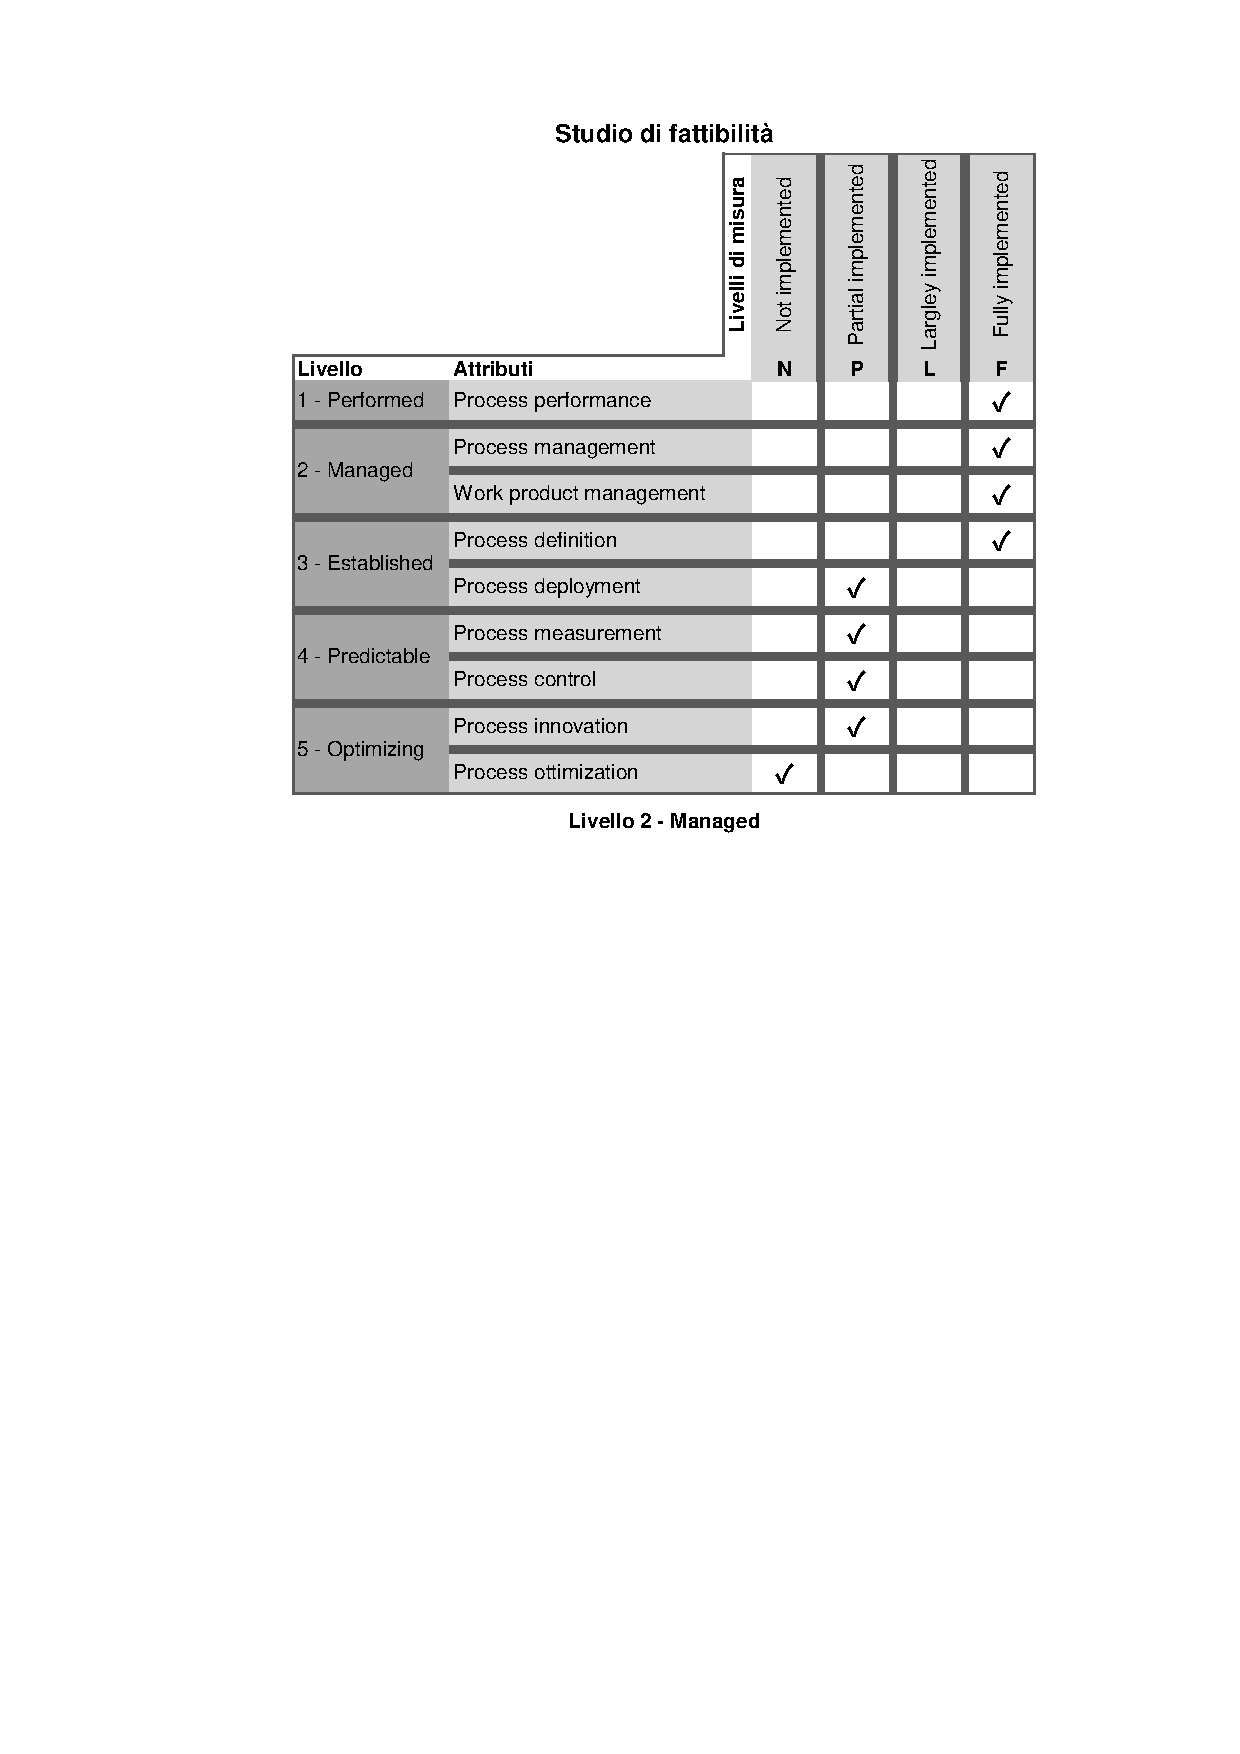
\includegraphics[scale=1]{images/resoconto/RR/studiodifattibilita-RR.pdf}
	\caption{Valori ISO/IEC 15504 Studio di fattibilità}	
\end{figure}
\newpage
\subparagraph{Norme di progetto}
\noindent
\begin{figure}[H]
	\centering
	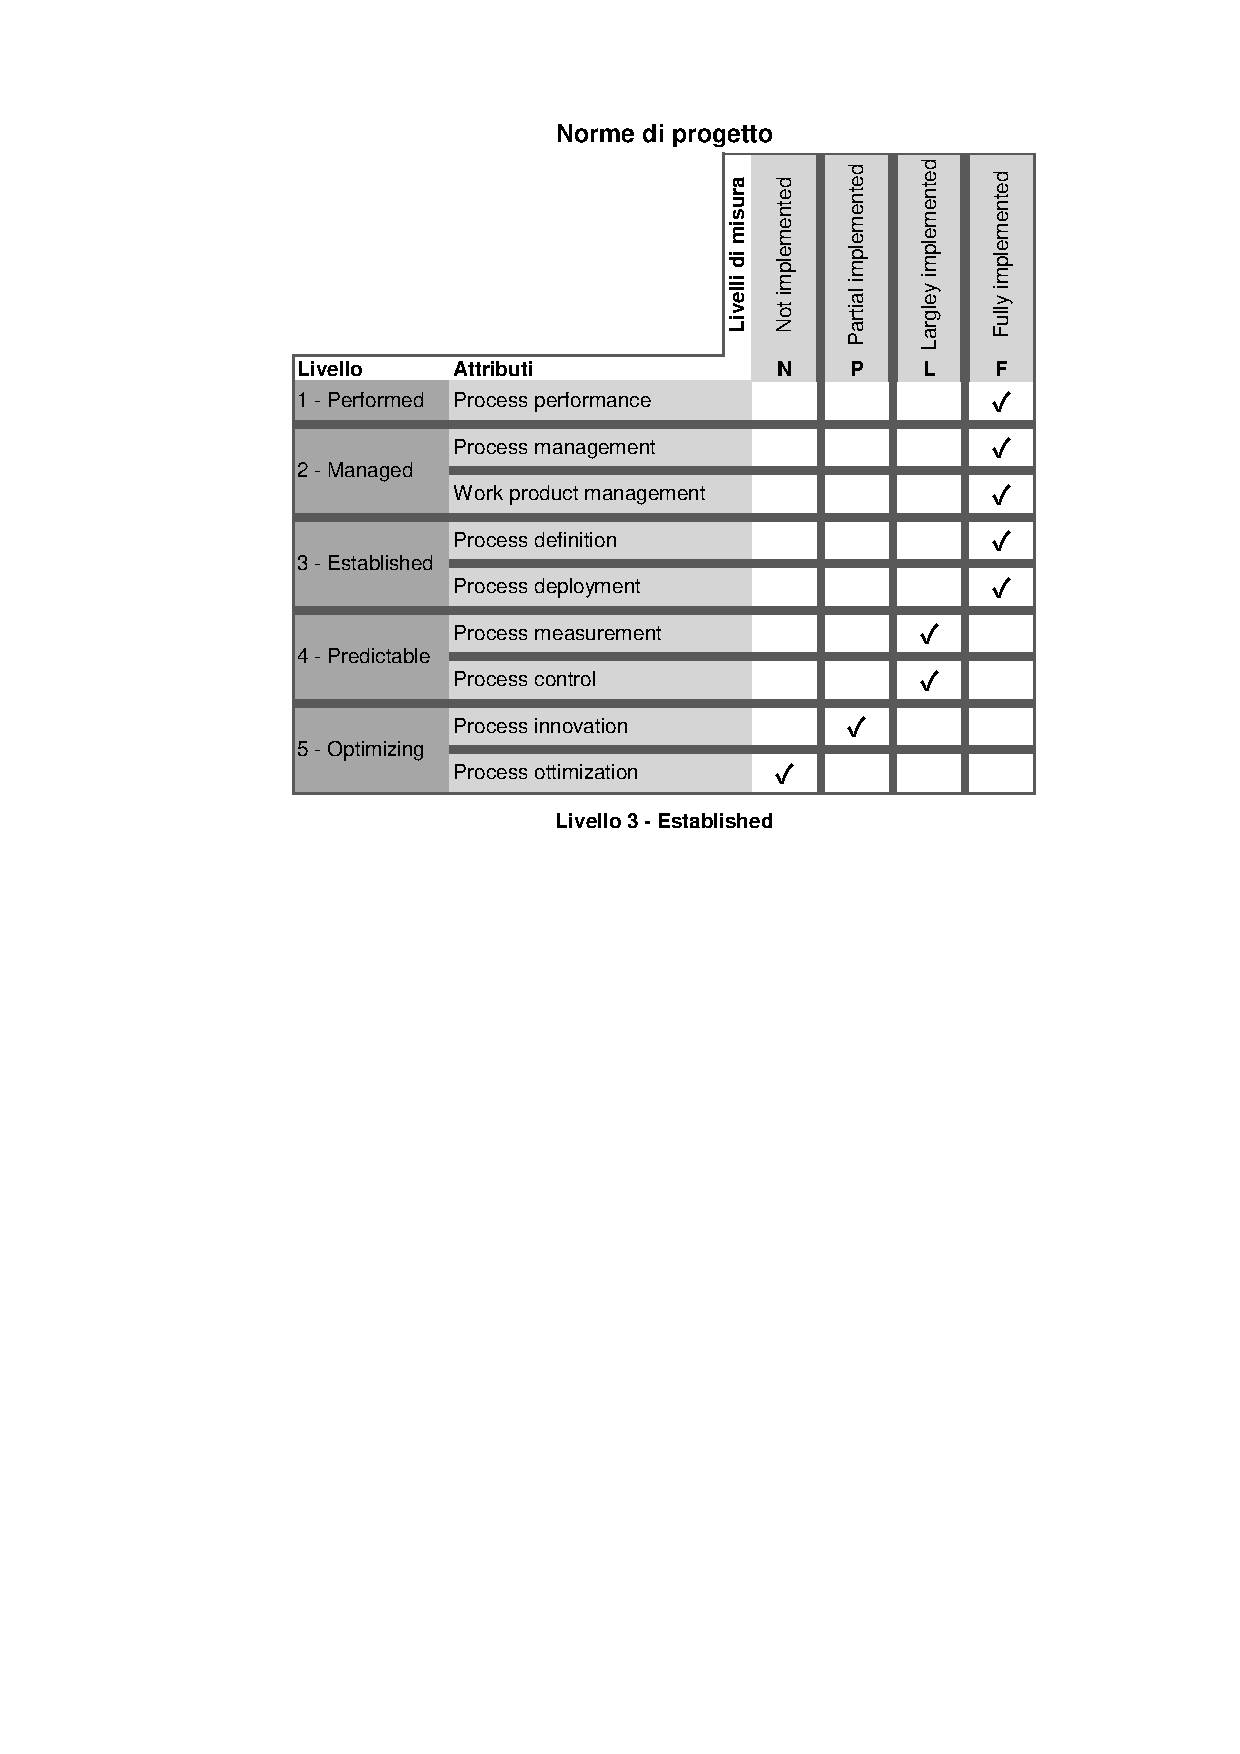
\includegraphics[scale=1]{images/resoconto/RR/normediprogetto-RR.pdf}
	\caption{Valori ISO/IEC 15504 Norme di progetto}	
\end{figure}
\newpage
\subparagraph{Analisi dei requisiti}
\noindent
\begin{figure}[H]
	\centering
	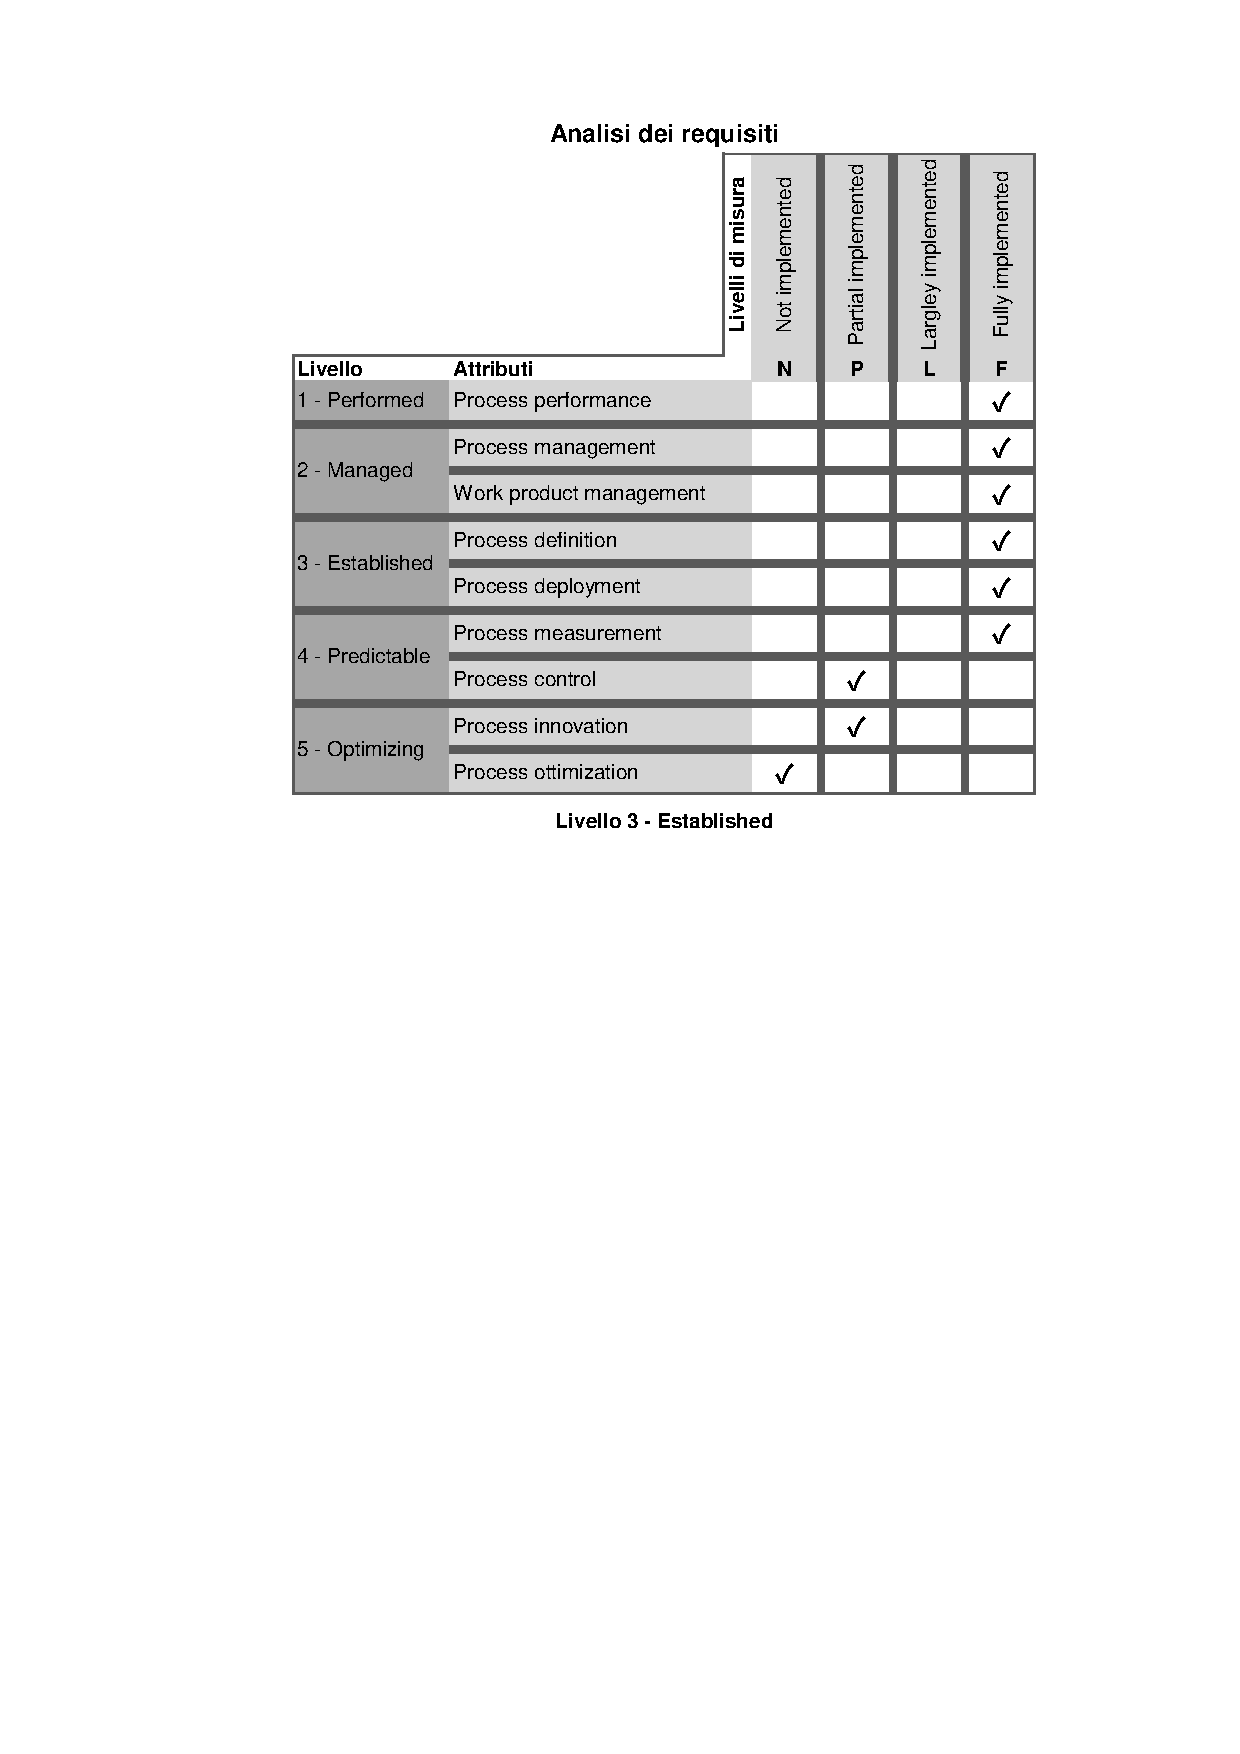
\includegraphics[scale=1]{images/resoconto/RR/analisideirequisiti-RR.pdf}
	\caption{Valori ISO/IEC 15504 Analisi dei requisiti}
\end{figure}
\newpage
\subparagraph{Pianificazione di progetto}
\noindent
\begin{figure}[H]
	\centering
	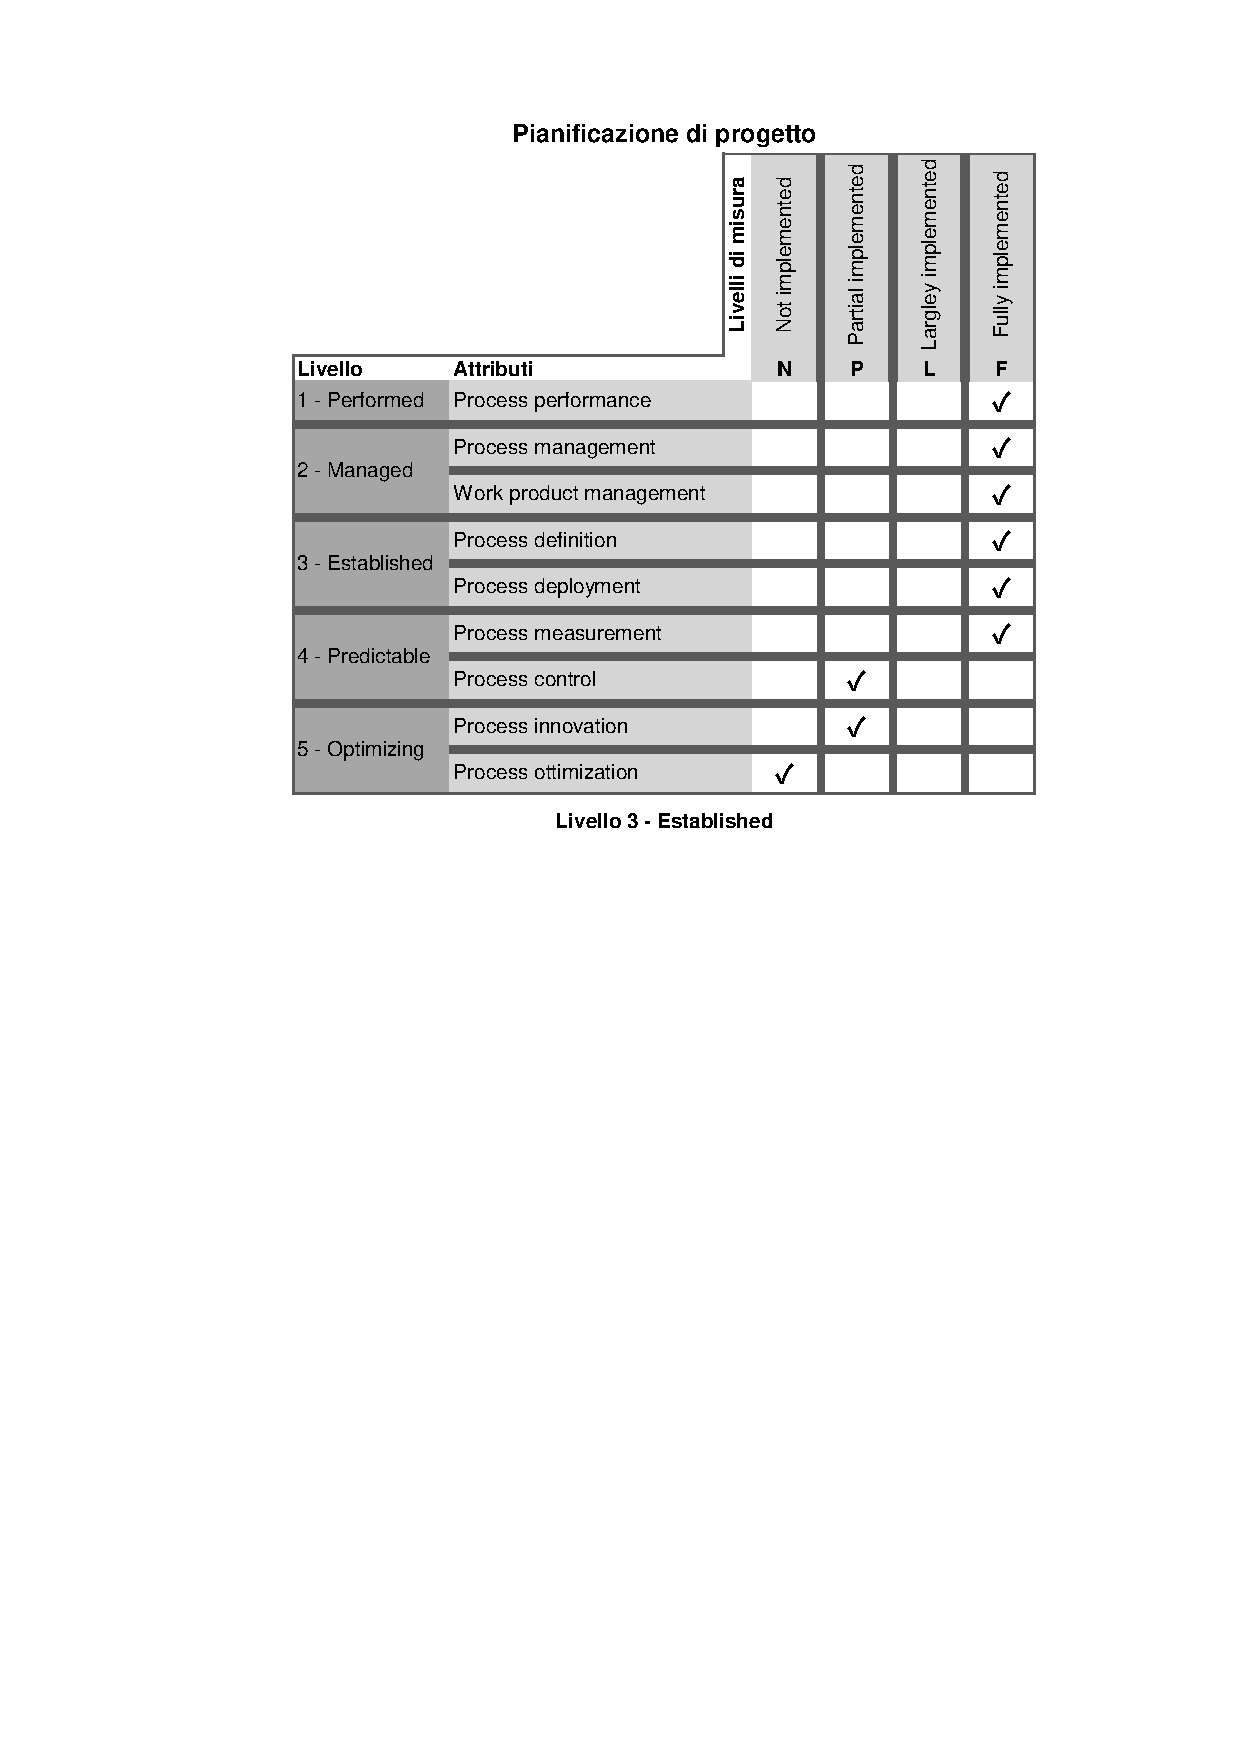
\includegraphics[scale=1]{images/resoconto/RR/pianificazioneprogetto-RR.pdf}
	\caption{Valori ISO/IEC 15504 Pianificazione di progetto}	
\end{figure}
\newpage
\subparagraph{Pianificazione di qualifica}
\noindent
\begin{figure}[H]
	\centering
	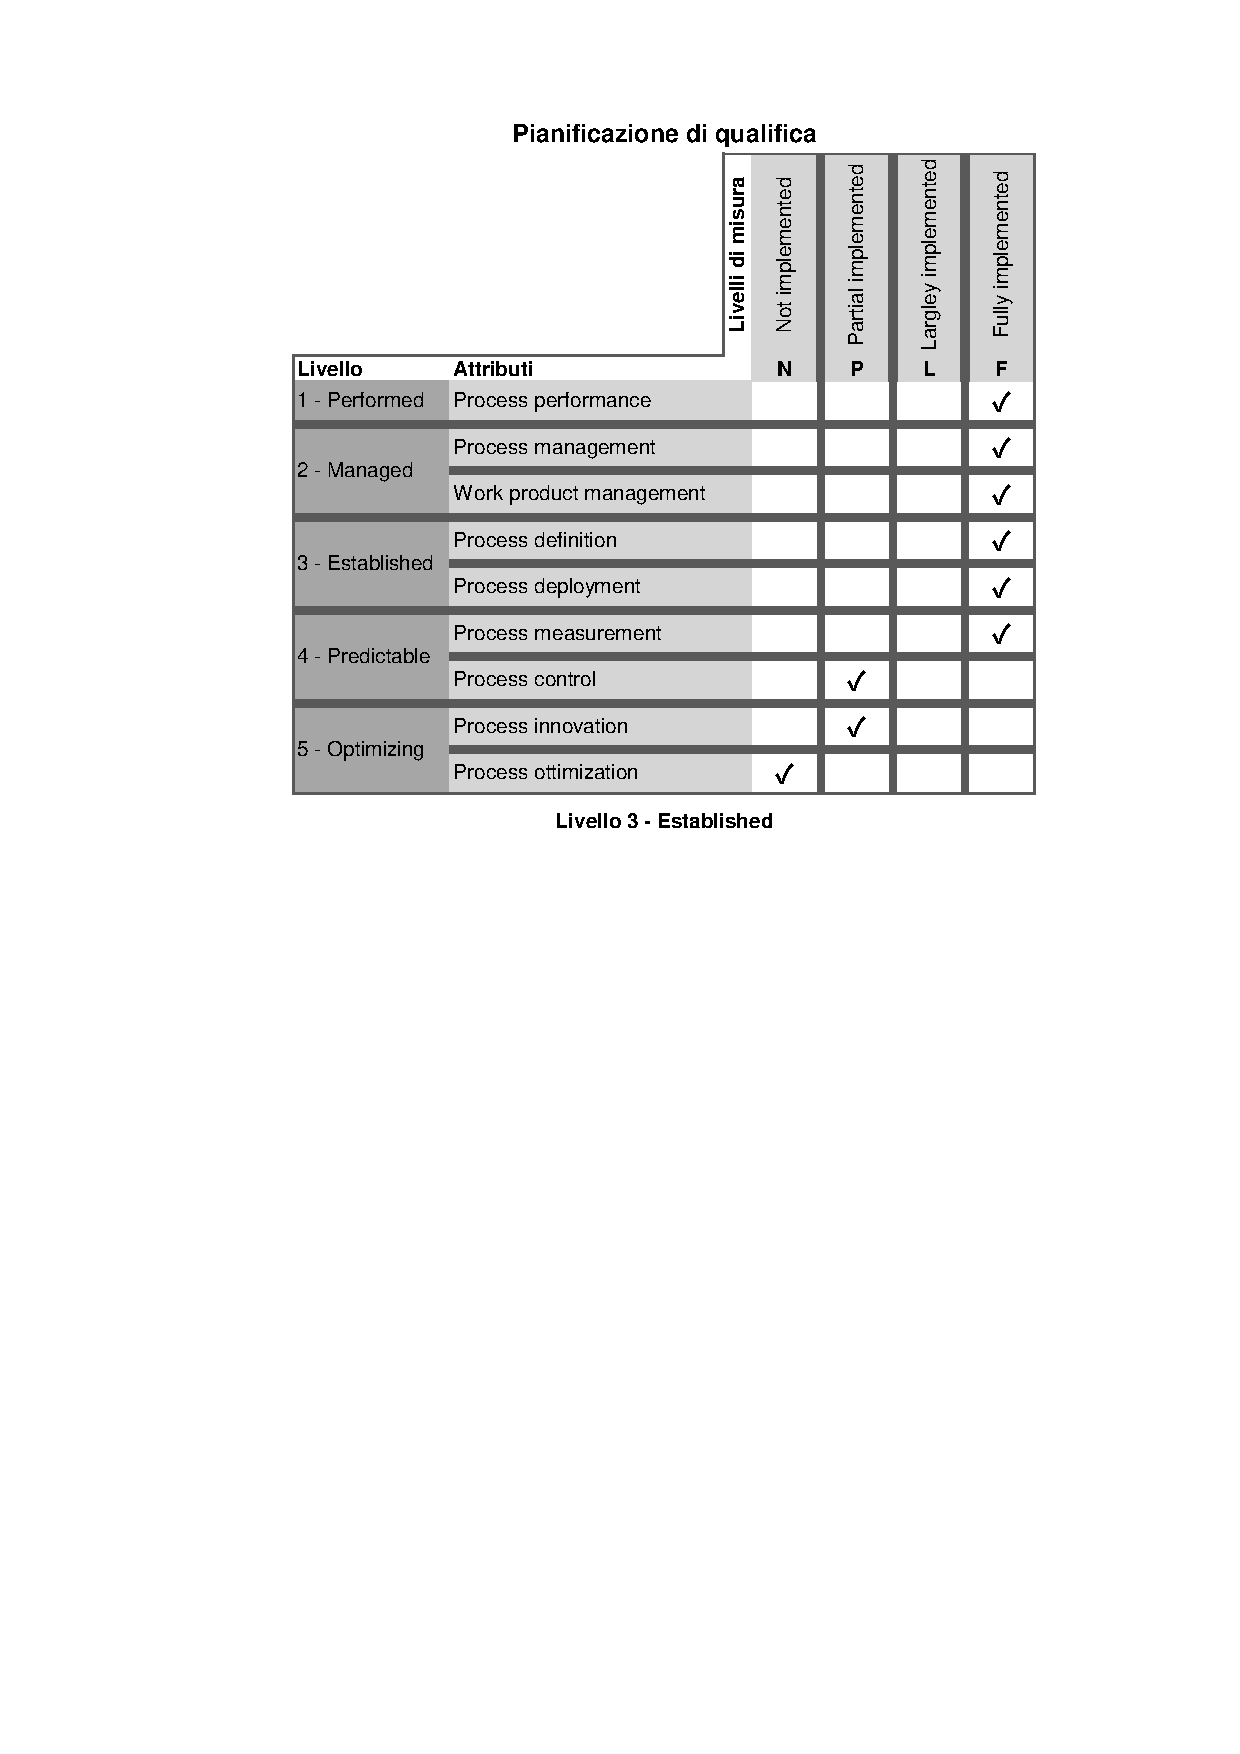
\includegraphics[scale=1]{images/resoconto/RR/pianificazionequalifica-RR.pdf}
	\caption{Valori ISO/IEC 15504 Pianificazione di qualifica}	
\end{figure}
\newpage

\subparagraph{Grafico riassuntivo}
Nel seguente grafico possiamo visualizzare una rappresentazione dei livelli raggiunti da ciascun processo implementato e quindi valutato durante il periodo della revisione dei requisiti. 

\begin{figure}[H]
	\centering
	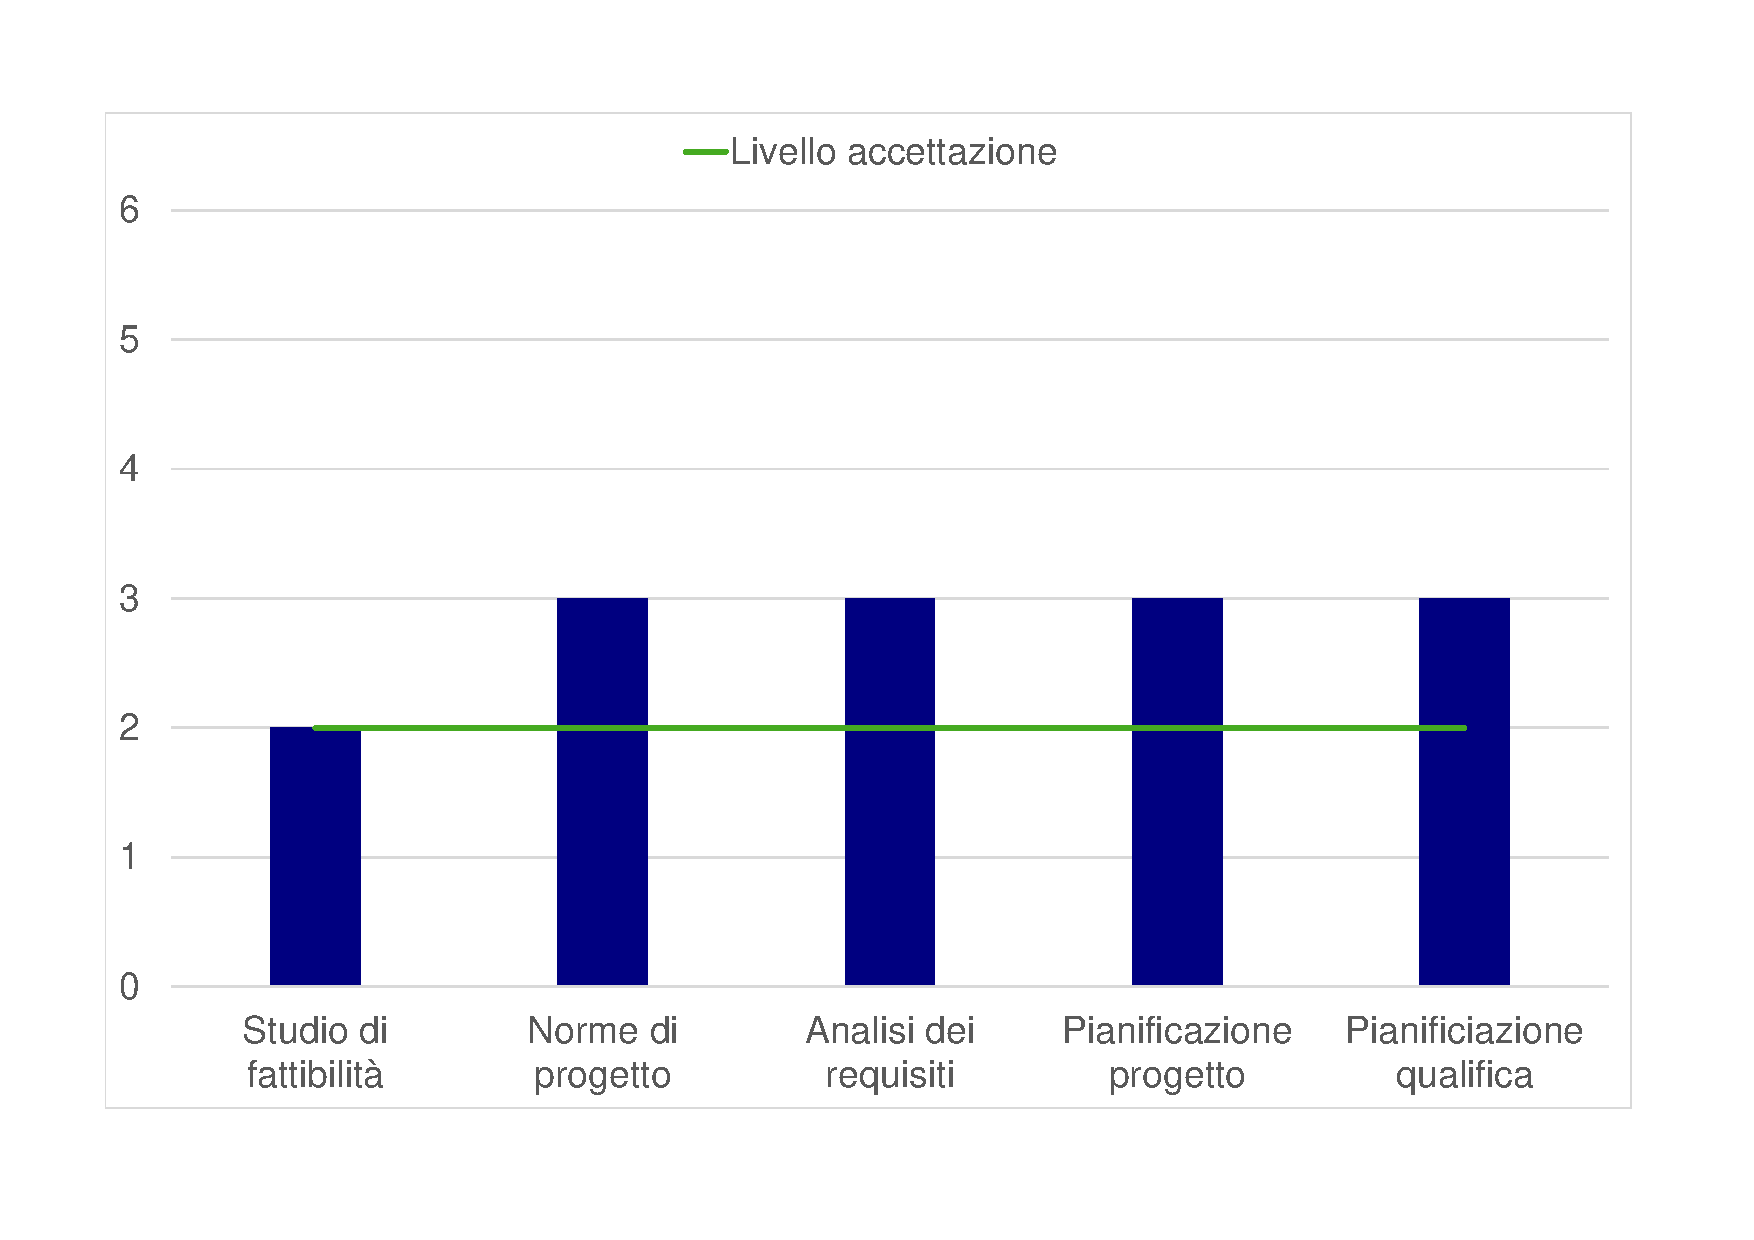
\includegraphics[scale=0.5]{images/resoconto/RR/chart-RR.pdf}
	\caption{Riassunto valori processi RR}
\end{figure}

\newpage
\paragraph{Revisione di Progettazione}
\noindent \\ 
Di seguito riportiamo le misurazioni dei processi più significativi sviluppati durante il periodo di Revisione di Progettazione. Tali valori sono stati raccolti secondo la metrica MPC1 che fa riferimento alle linee guida dettate dallo standard ISO/IEC 15504.
\subparagraph{Normazione}
\noindent
\begin{figure}[H]
	\centering
	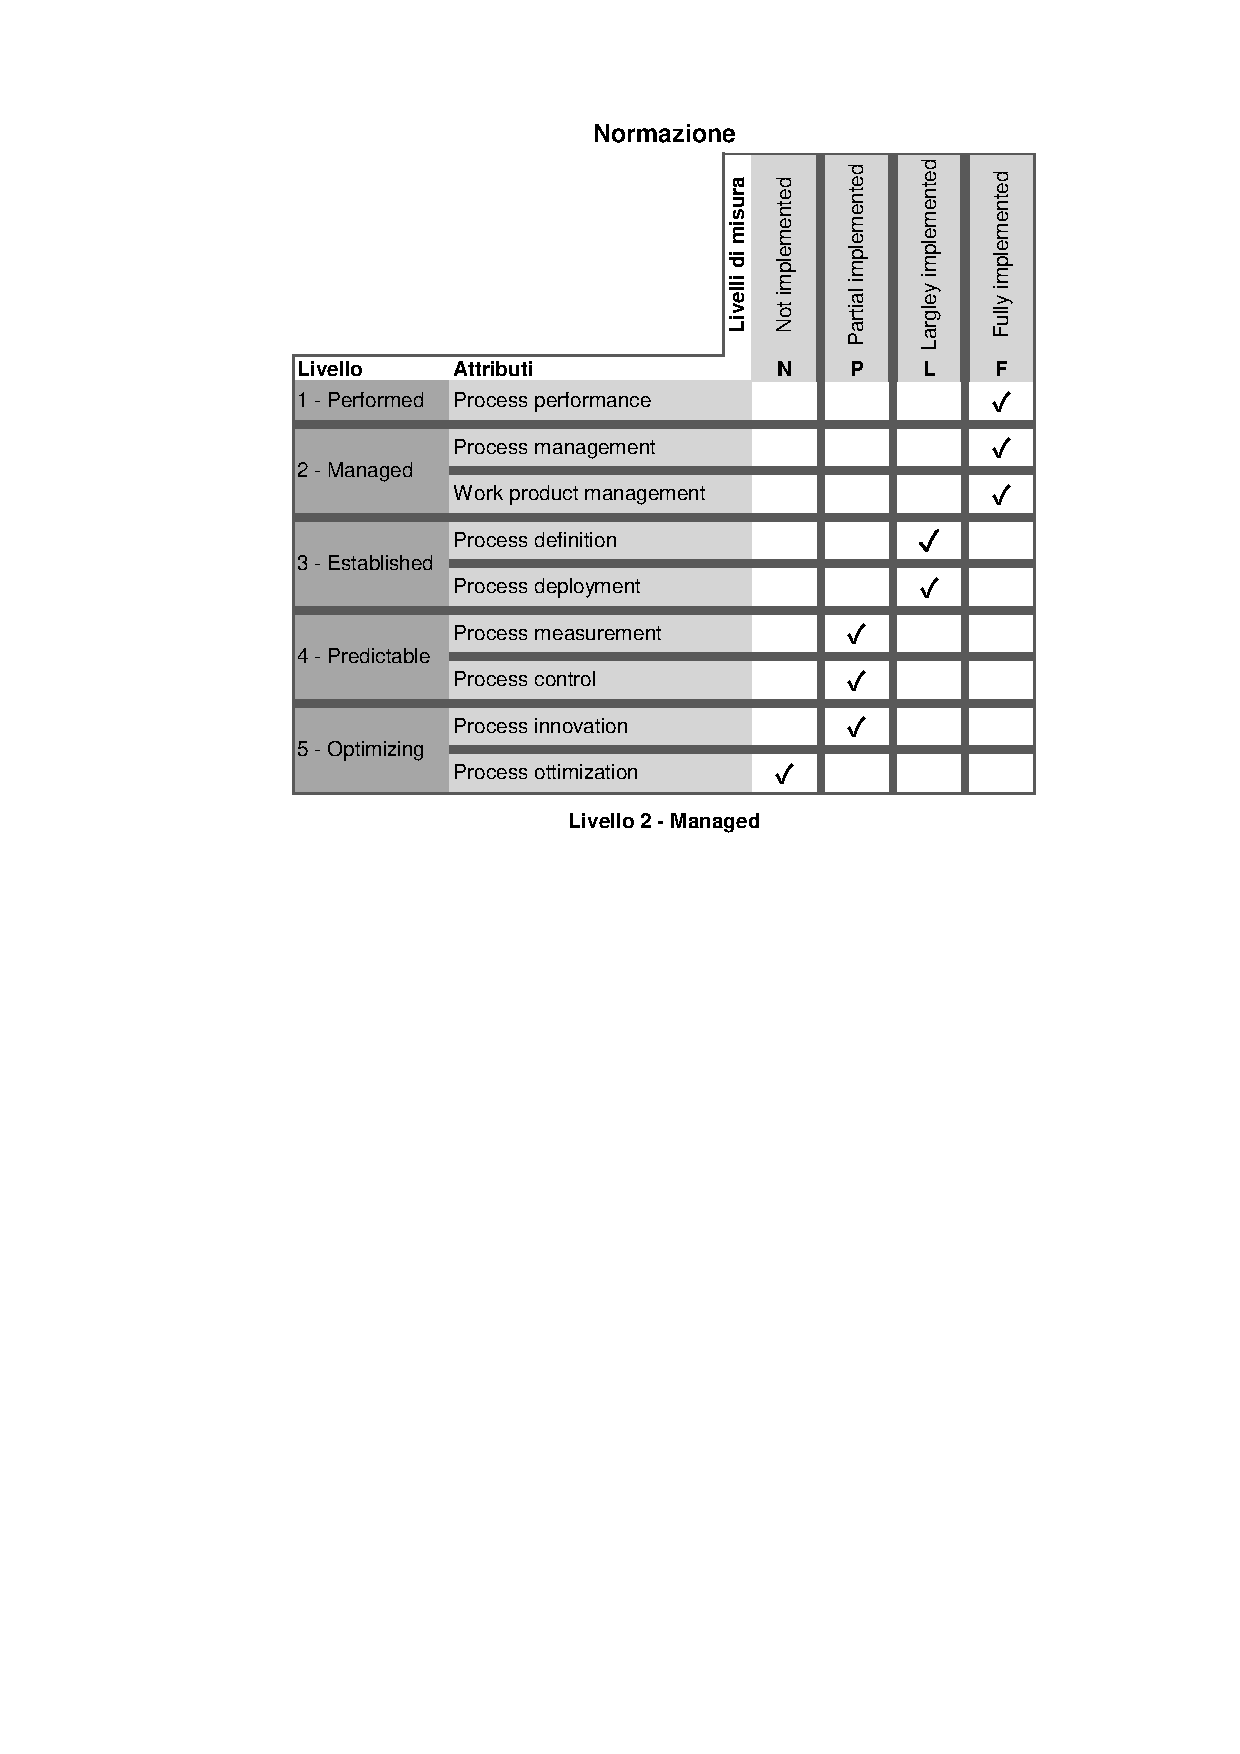
\includegraphics[scale=1]{images/resoconto/RP/normazione-RP.pdf}
	\caption{Valori ISO/IEC 15504 Pianificazione progetto}	
\end{figure}
\newpage
\subparagraph{Analisi dei requisiti}
\noindent
\begin{figure}[H]
	\centering
	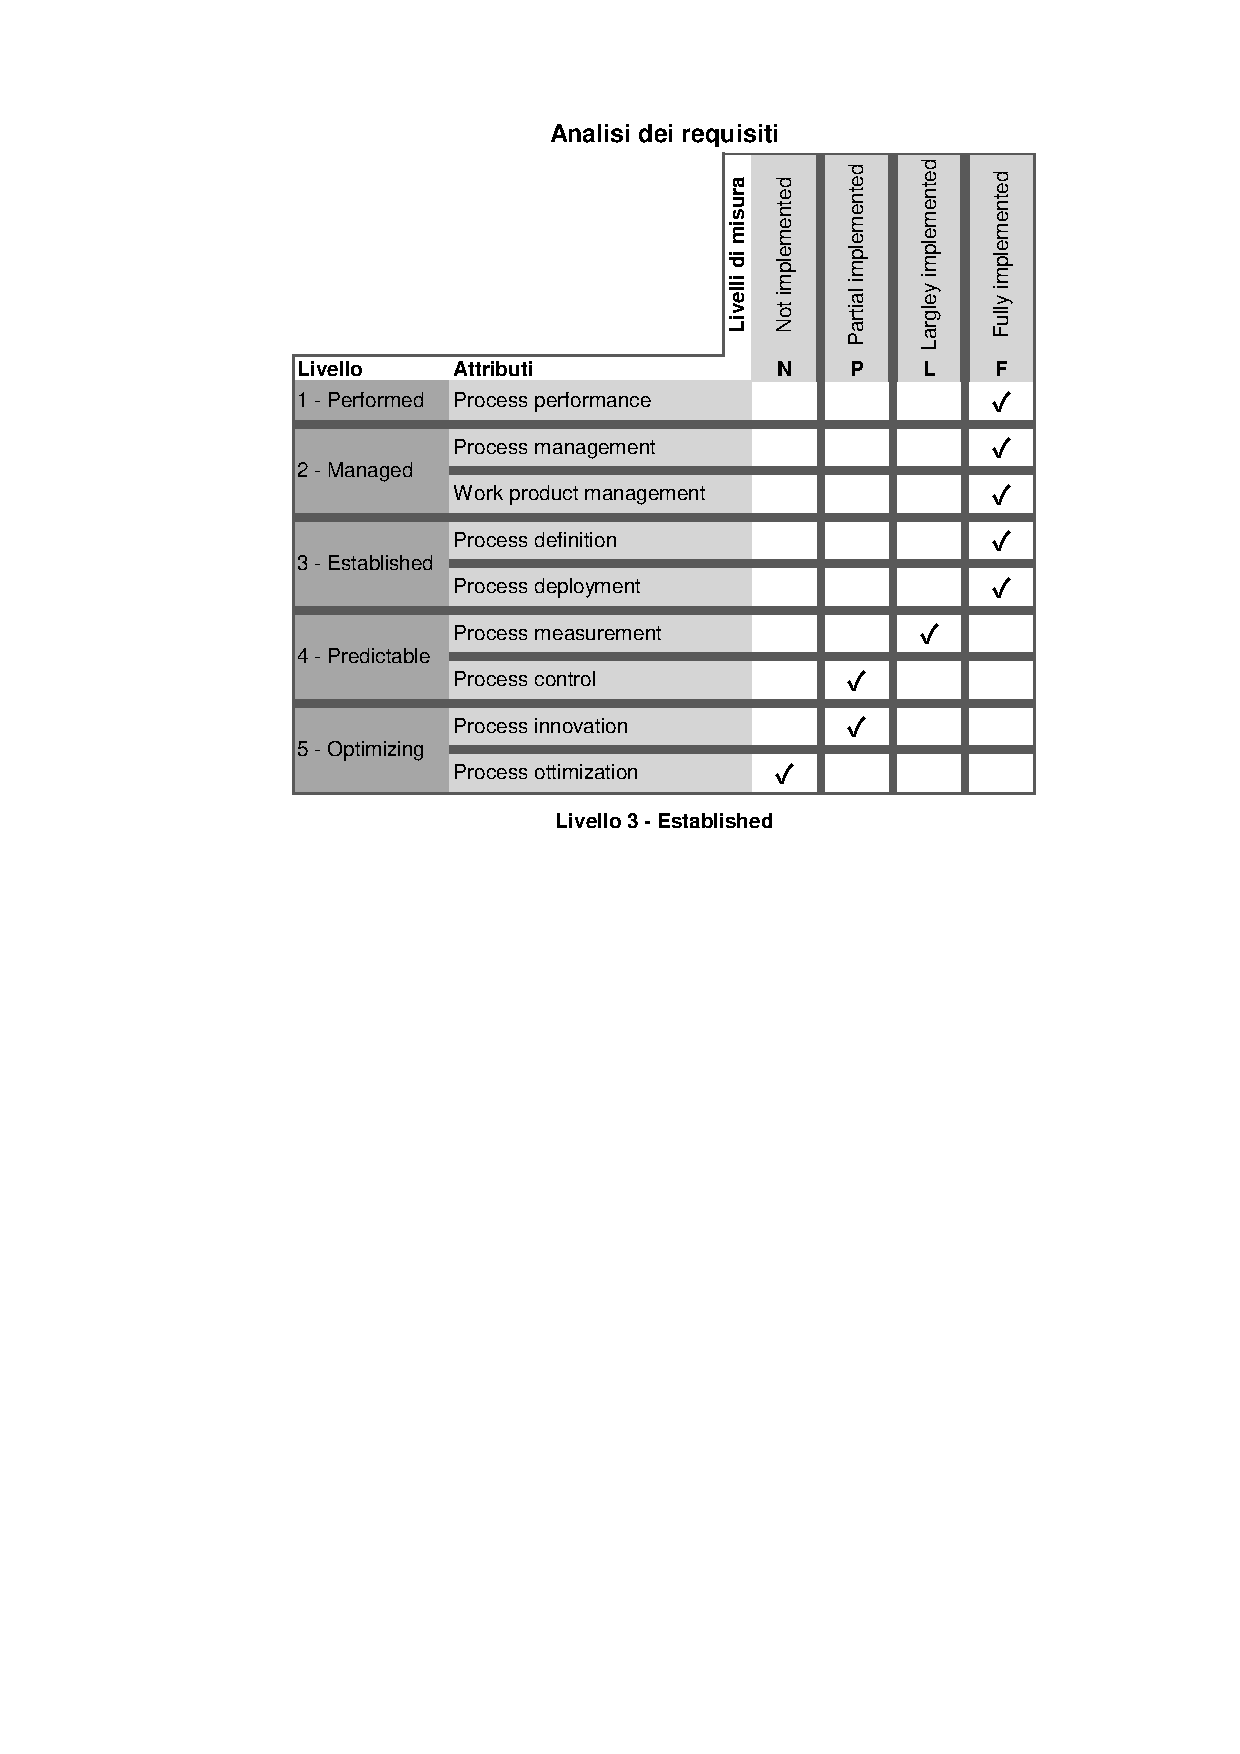
\includegraphics[scale=1]{images/resoconto/RP/analisideirequisiti-RP.pdf}
	\caption{Valori ISO/IEC 15504 Analisi dei requisiti}	
\end{figure}
\newpage
\subparagraph{Progettazione}
\noindent
\begin{figure}[H]
	\centering
	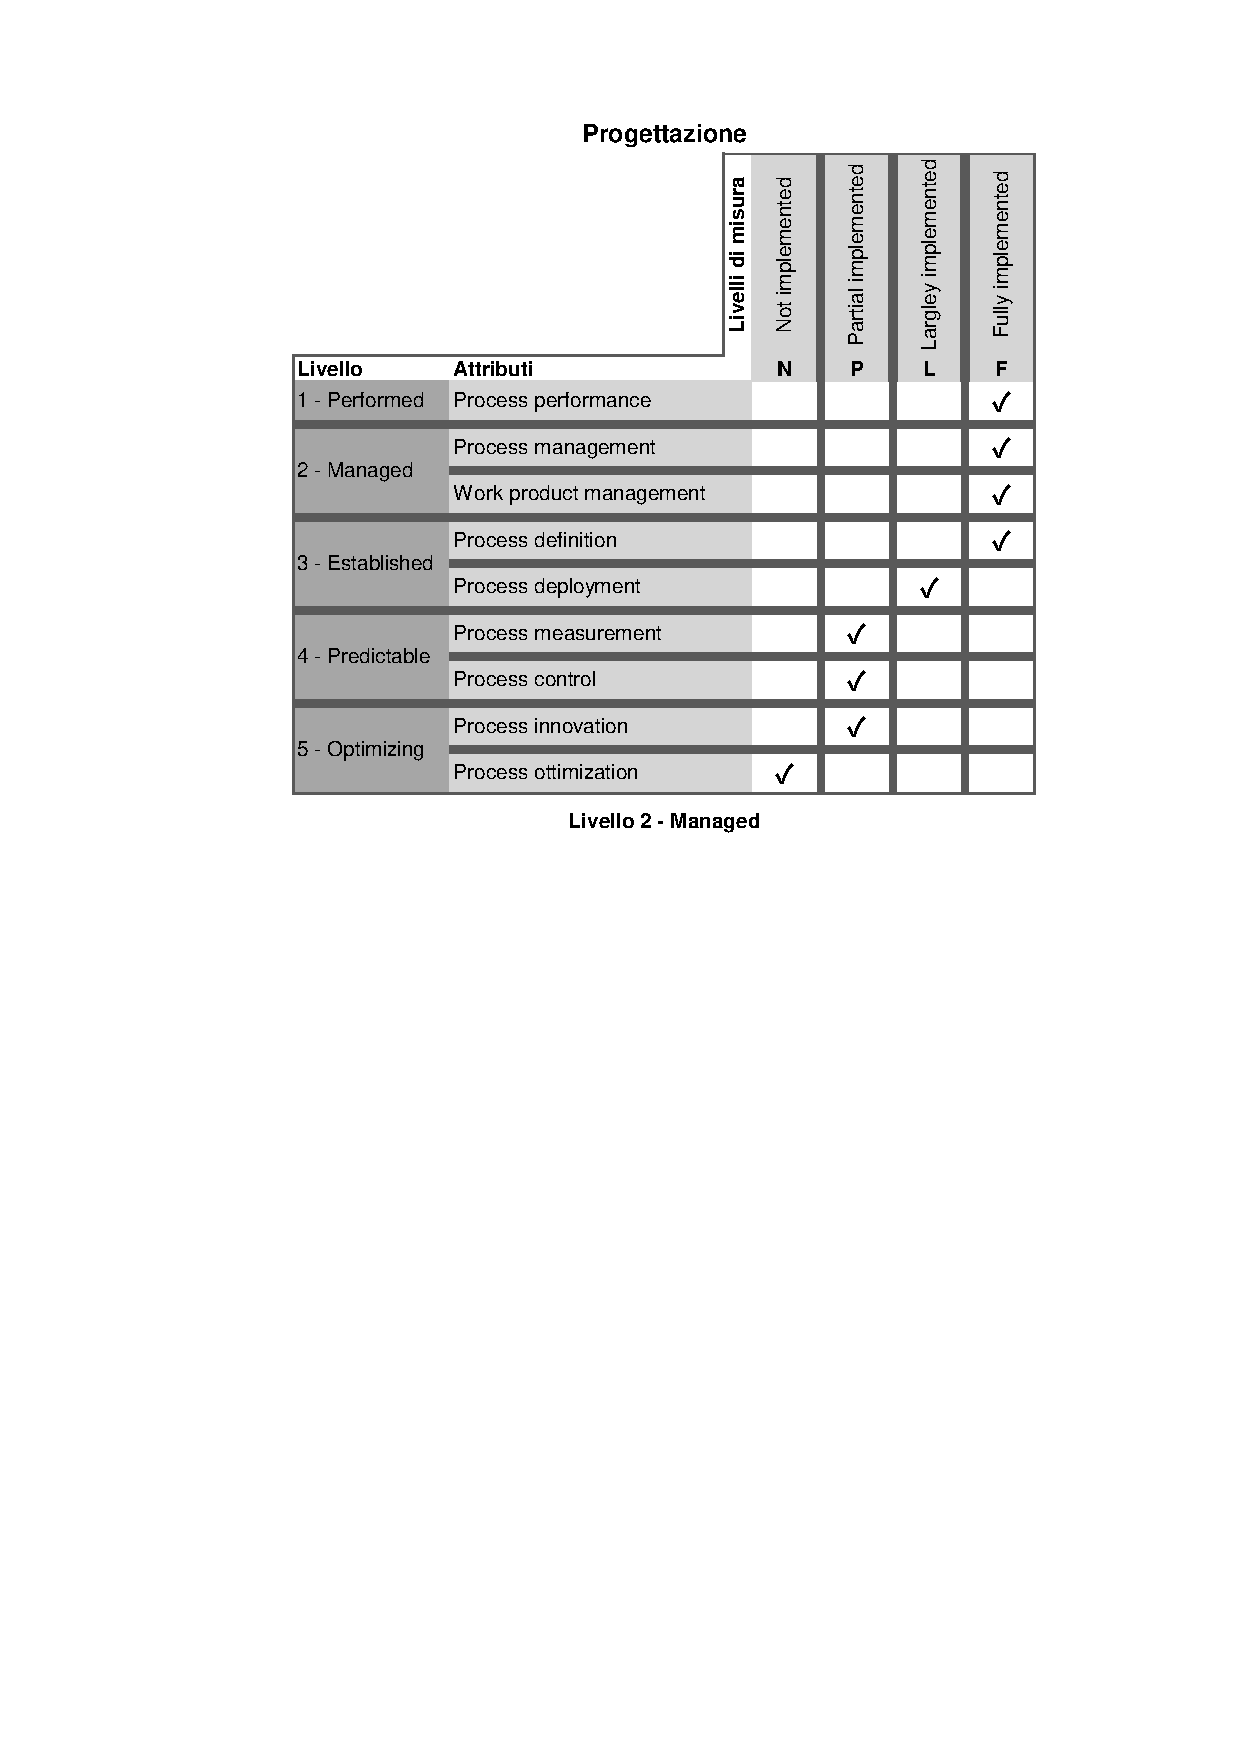
\includegraphics[scale=1]{images/resoconto/RP/progettazione-RP.pdf}
	\caption{Valori ISO/IEC 15504 Progettazione}	
\end{figure}
\newpage
\subparagraph{Documentazione}
\noindent
\begin{figure}[H]
	\centering
	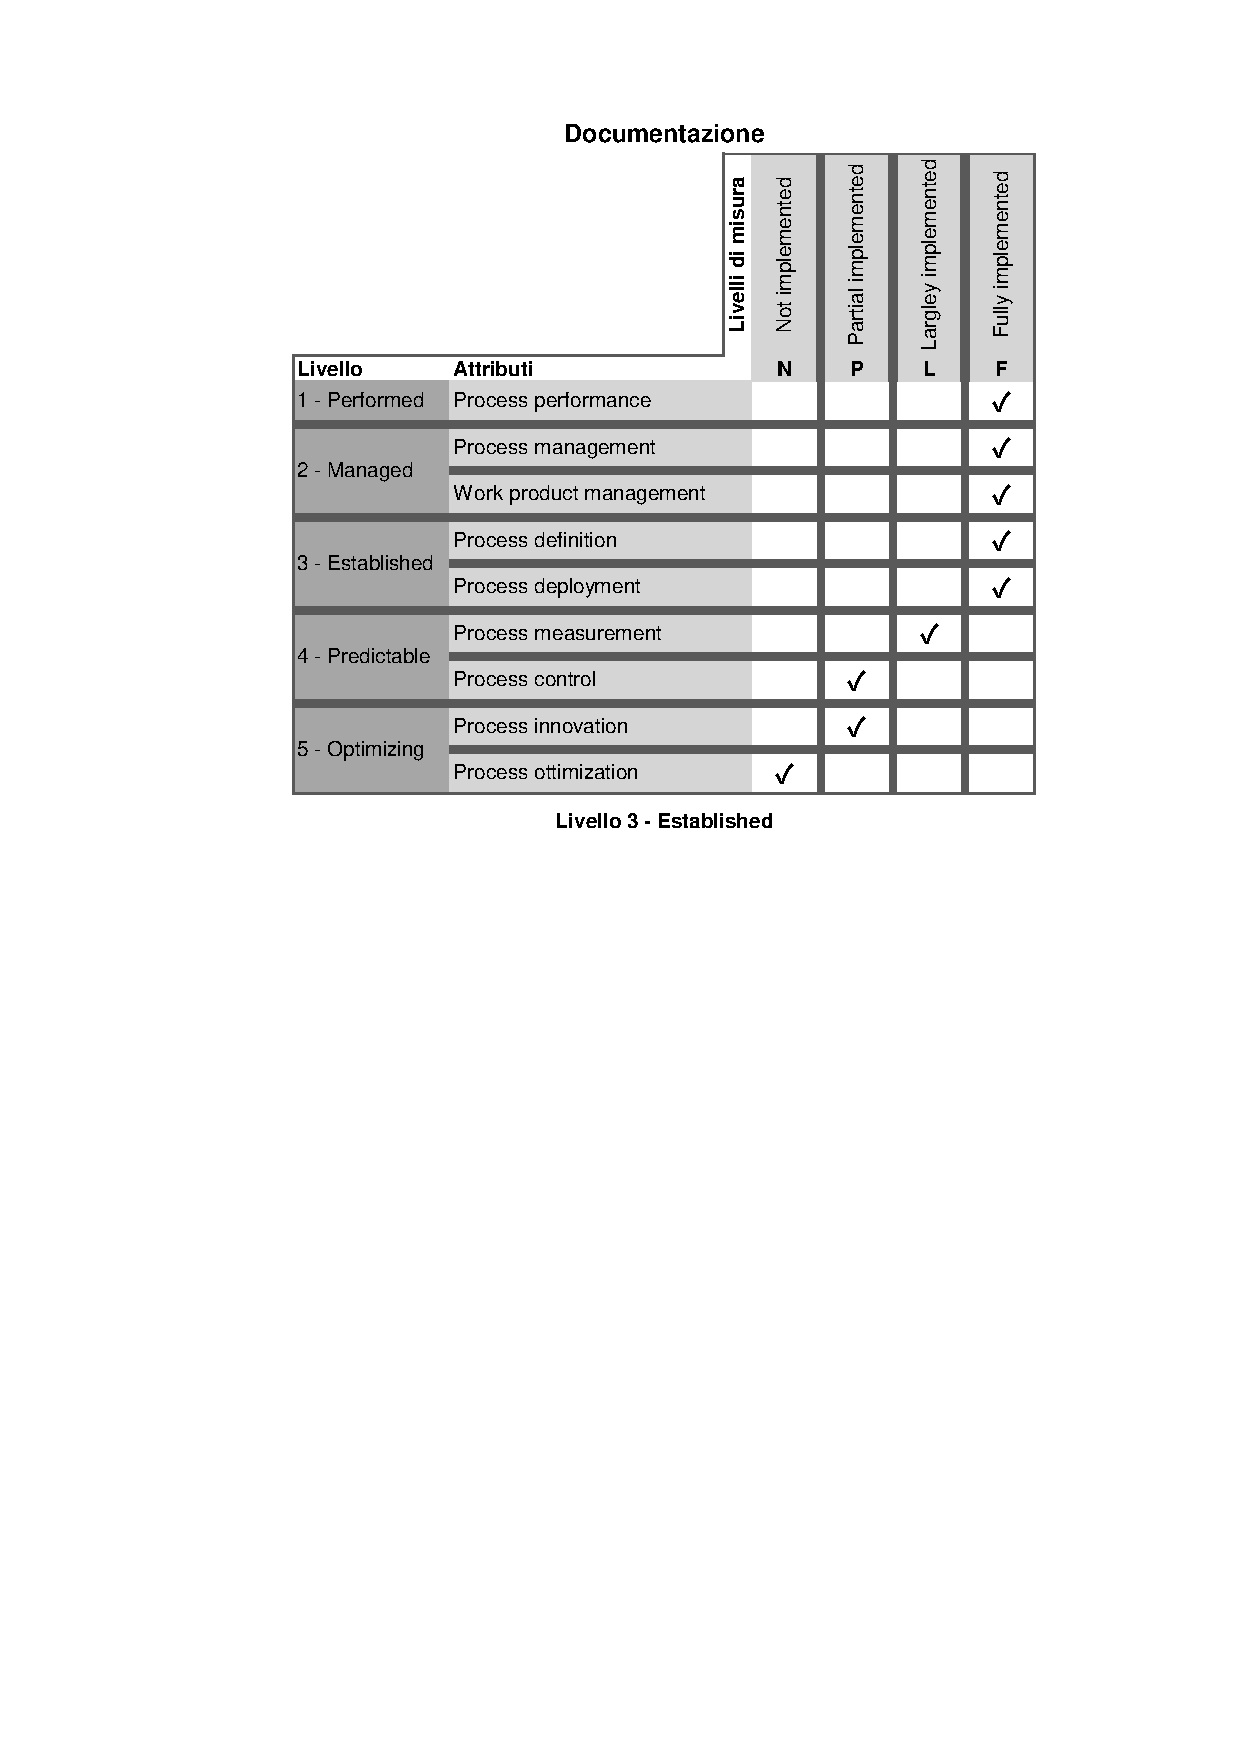
\includegraphics[scale=1]{images/resoconto/RP/documentazione-RP.pdf}
	\caption{Valori ISO/IEC 15504 Documentazione}	
\end{figure}
\newpage
\subparagraph{Pianificazione progetto}
\noindent
\begin{figure}[H]
	\centering
	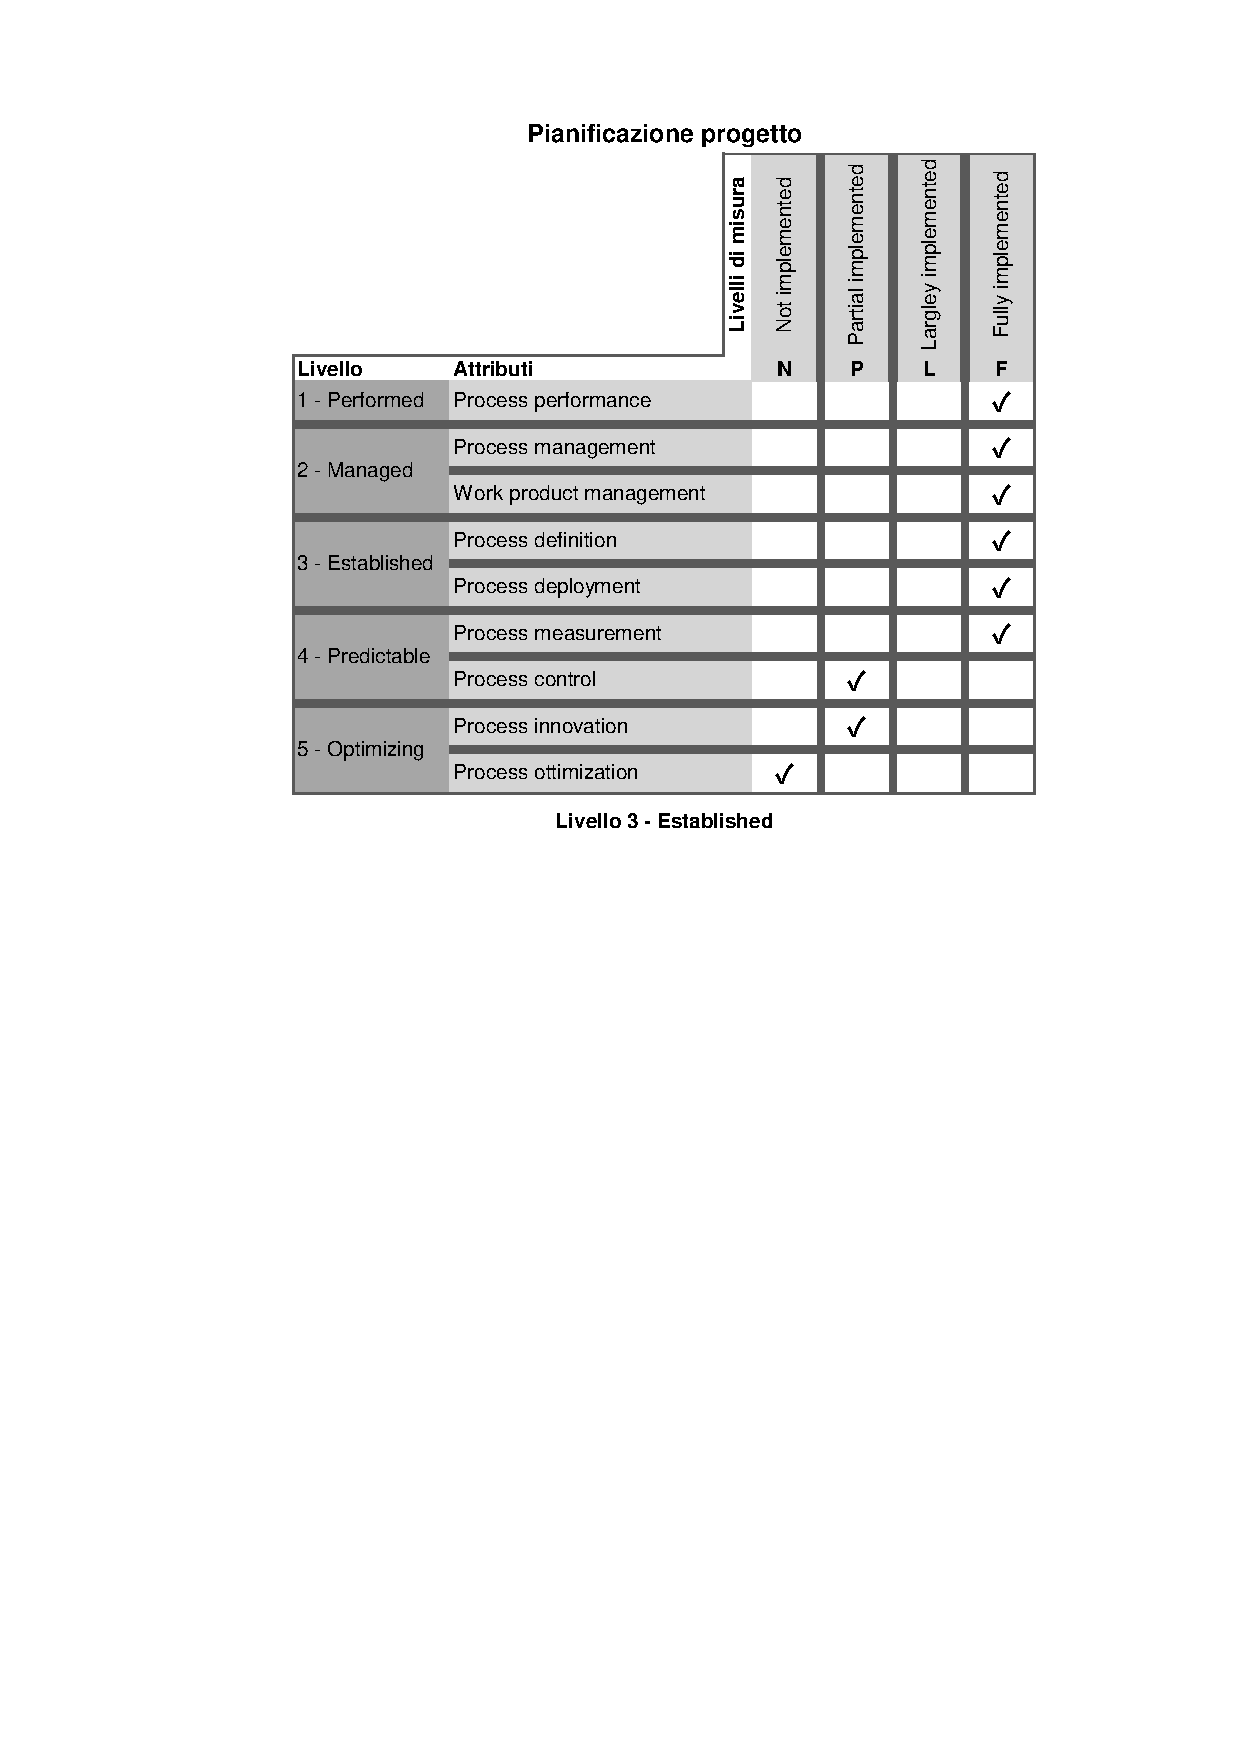
\includegraphics[scale=1]{images/resoconto/RP/pianificazioneprogetto-RP.pdf}
	\caption{Valori ISO/IEC 15504 Pianificazione progetto}	
\end{figure}
\newpage
\subparagraph{Ricerca delle tecnologie}
\noindent
\begin{figure}[H]
	\centering
	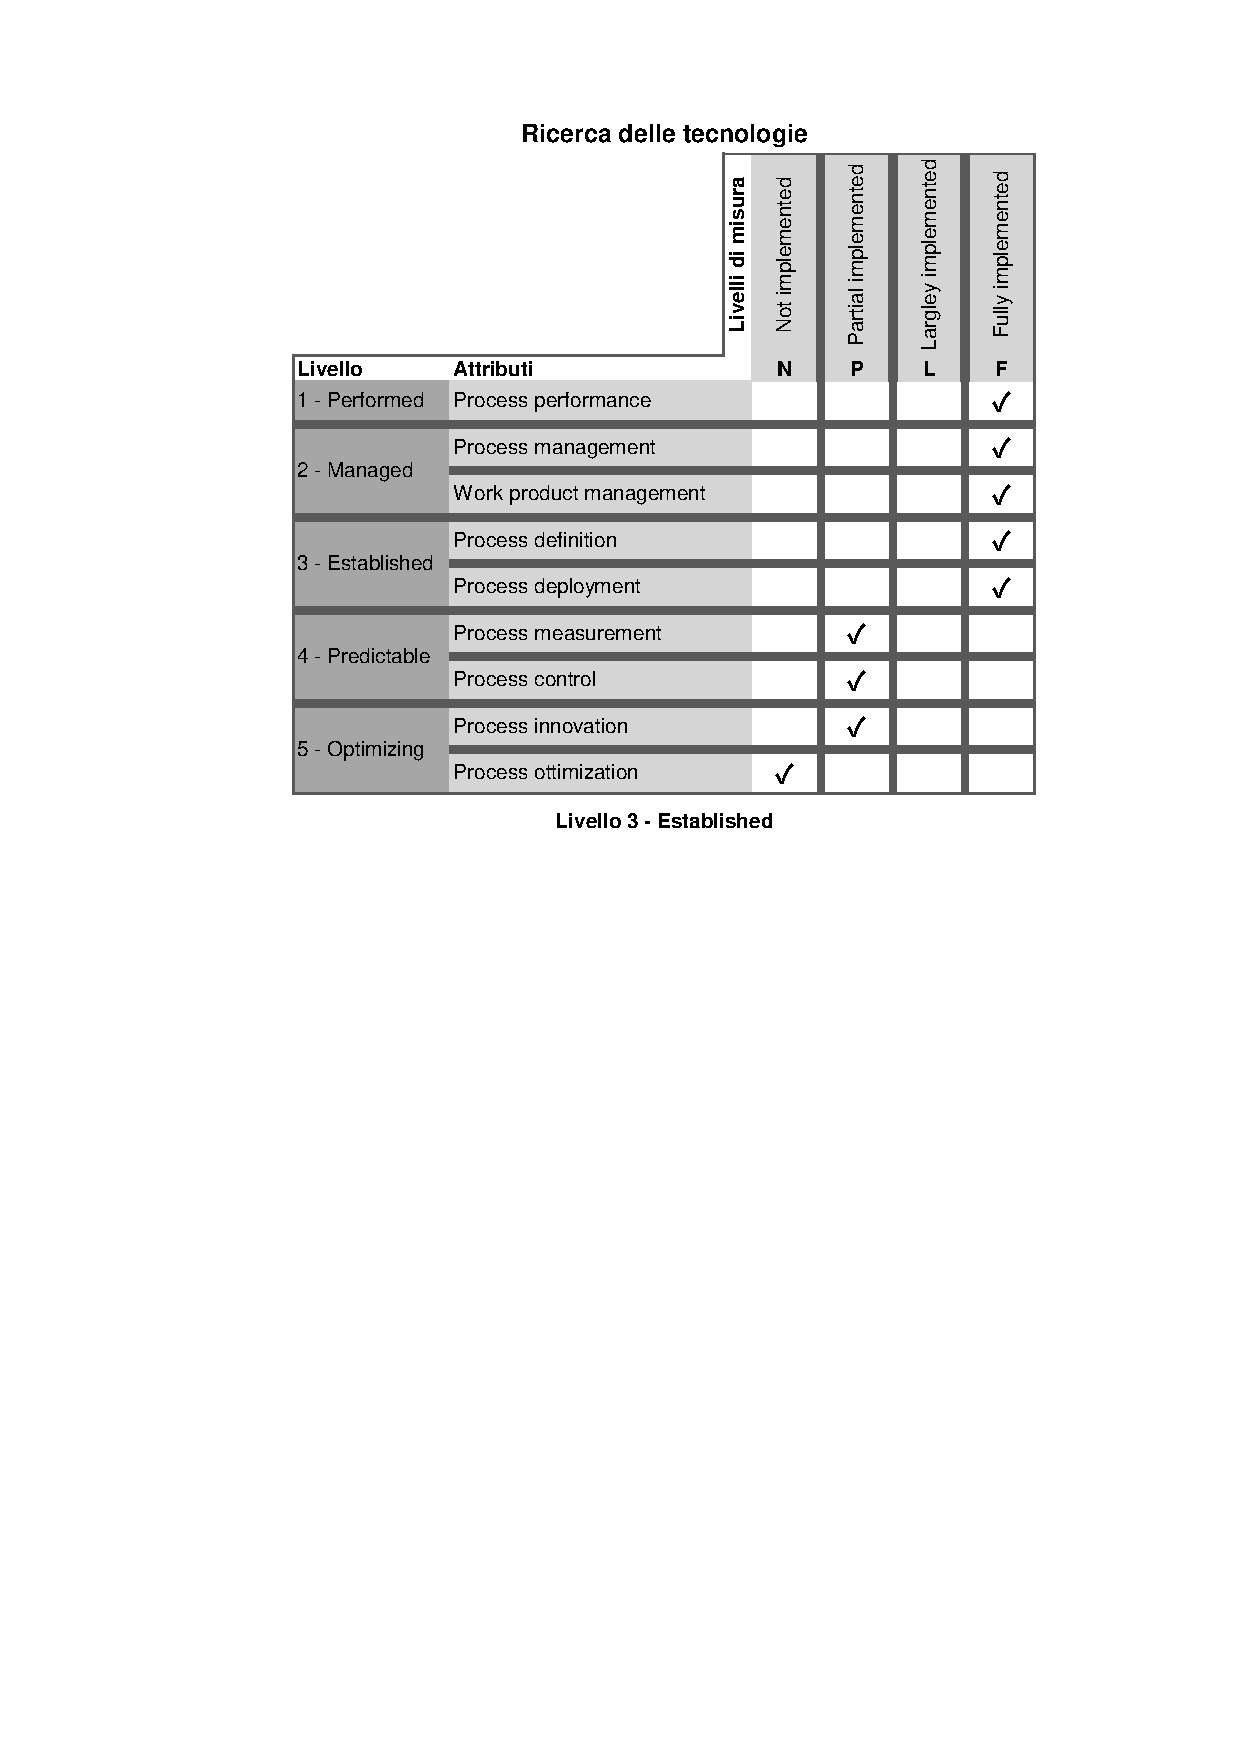
\includegraphics[scale=1]{images/resoconto/RP/ricercadelletecnologie-RP.pdf}
	\caption{Valori ISO/IEC 15504 Ricerca delle tecnologie}	
\end{figure}
\newpage

\subparagraph{Grafico riassuntivo}
Nel seguente grafico possiamo visualizzare una rappresentazione dei livelli raggiunti da ciascun processo implementato e quindi valutato durante il periodo della revisione di progetto. 

\begin{figure}[H]
	\centering
	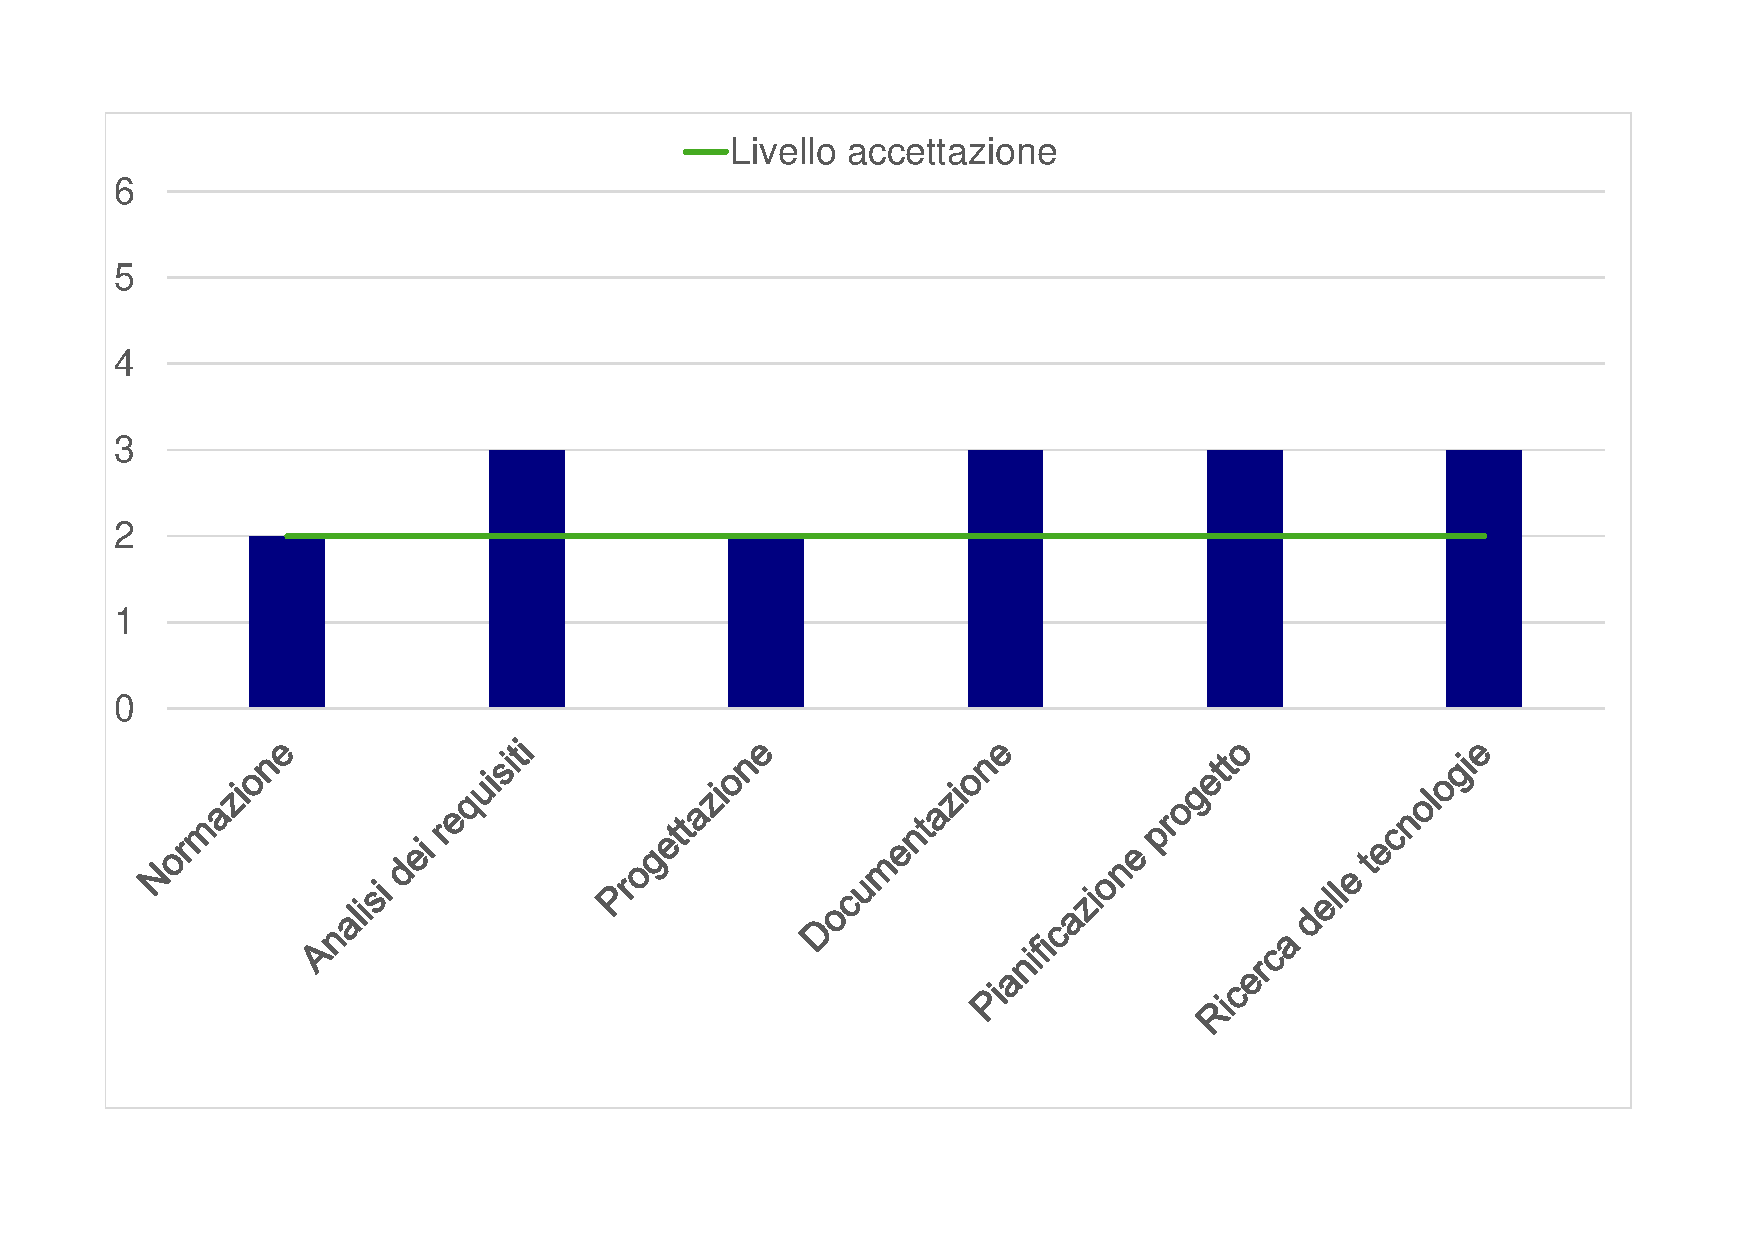
\includegraphics[scale=0.5]{images/resoconto/RP/chart-RP.pdf}
	\caption{Riassunto valori processi RP}	
\end{figure}

\newpage
\section{ISO/IEC 15504}
Lo standard ISO/IEC 15504, comunemente chiamato SPICE (acronimo di Software Process Improvement and Capability Determination), viene utilizzato per eseguire una valutazione concreta della qualità dei processi, inoltre permette la misurazione della capability dei processi, ovvero l'abilità con cui esso raggiunge l'obiettivo prefissato. Per eseguire queste misurazioni lo standard offre nove attributi da associare ai processi, ognuno dei quali misura un particolare aspetto della maturità del processo:
\begin{itemize}
	\item \textbf{Process performance:} è una misura del grado con cui è stato raggiunto lo scopo del processo. Il completo raggiungimento di quest'attributo è dato dal fatto che il processo raggiunge gli obiettivi prefissati.
	\item \textbf{Perfomance management:} è una misura del grado con il quale viene gestita l'organizzazione per il raggiungimento dello scopo del processo. Il processo è pianificato e monitorato. Le responsabilità per la realizzazione del processo sono assegnate e comunicate. Le risorse necessarie per il processo sono disponibili, allocate e utilizzate. 
	\item \textbf{Work product management:} è una misura del grado con il quale i risultati prodotti dal processo vengono appropriatamente gestiti. I requisiti dei risultati della documentazione e del controllo del processo sono definiti e i risultati devono essere appropriatamente documentati e controllati. I risultati del processo sono sottoposti a verifica e a correzione se necessario.
	\item \textbf{Process definition:} è una misura del grado con cui uno standard di processo è mantenuto (utilizzato) a supporto dell'implementazione del processo. Gli elementi fondamentali dello standard da utilizzare sono descritti e la sequenza di operazioni richieste dallo standard è definita. Le competenze, i ruoli, le infrastrutture e l'ambiente di lavoro per realizzare il processo fanno parte dello standard. I metodi di monitoraggio del processo sono definiti.
	\item \textbf{Process deployment:} è una misura del grado con il quale lo standard di processo viene effettivamente distribuito come un processo definito in grado di raggiungere i propri obiettivi. Le responsabilità e i ruoli per utilizzare lo standard sono assegnati e comunicati, le risorse, le infrastrutture e l'ambiente di lavoro, necessarie per l'applicazione dello standard, sono disponibili allocate e utilizzate. Vengono raccolti e analizzati dati per dimostrare l'adeguatezza e l'efficacia del processo.
	\item \textbf{Process measurement:} è una misura del grado con il quale i risultati delle misurazioni sono utilizzati per garantire il raggiungimento degli obiettivi del processo. Vengono definiti degli obiettivi di qualità basati sulle misurazioni. I risultati delle misurazioni sono raccolti analizzati e documentati per verificare che gli obiettivi di qualità siano rispettati.
	\item \textbf{Process control:} è una misura del grado con il quale il processo è quantitativamente gestito per produrre un processo che sia stabile, abile e previdibile entro limiti definiti. Analisi e tecniche di controllo vengono applicate. Sono stabiliti dei limiti di variazione per i risultati delle misurazioni. Vengono intraprese delle azioni correttive se necessario. 
	\item \textbf{Process innovation:} è una misura del grado con il quale vengono identificate delle modifiche al processo attraverso l'analisi di cause comuni di variazione delle performance, e dalla ricerca di approcci innovativi alla definizione e all'implementazione del processo. Vengono definiti degli obiettivi di miglioramento. Vengono analizzati dei dati per identificare le cause comuni di variazione delle performance del processo e sucessivamente per identificare delle best-practice*.
	\item \textbf{Process optimization:} è una misura del grado con il quale delle modifiche alla definizione, gestione e alle prestazioni del processo si traducono in un impatto che porta a raggiungere rilevanti miglioramenti al processo. L'impatto dei cambiamenti proposti viene valutato rispetto agli obiettivi definiti dal processo e dallo standard di processo.
\end{itemize}
A questi attributi viene assegnato uno dei seguenti quattro livelli di misura:
\begin{itemize}
	\item \textbf{N not implemented:} non ci sono segni di raggiungimento dell'attributo.
	\item \textbf{P partial implemented:} esistono alcuni risultati dell'attributo in questione.
	\item \textbf{L largely implemented:} ci sono significanti segni di raggiungimento dell'attributo in questione.
	\item \textbf{F fully implemented:} viene identificato un pieno raggiungimento degli obiettvi dell'attributo
\end{itemize}
Infine sulla base delle valutazioni assegnate ad ogni attributo del processo, potrà essere valutato il grado complessivo di maturazione, il quale varierà sui seguenti sei valori:
\begin{itemize}
	\item \textbf{0 - Incomplete:} viene rilevato un fallimento generale nel conseguimento dell'obiettivo del processo. Non si identifica alcun prodotto o risultato. Un processo appartenente a questo livello non può essere associato ad alcun attributo.
	\item \textbf{1 - Performed:} lo scopo del processo è generalmente raggiunto, a prova di ciò sono identificabili dei prodotti risultanti dal processo. A questo livello il processo viene associato all' attributo Process performance.
	\item \textbf{2 - Managed:} il processo raggiunge dei risultati di qualità accettabile rispettando i tempi prestabiliti. Il risultato soddisfa tutti i requisiti e gli standard predefiniti. Un processo a questo livello è quindi gestito tramite pianificazione e controllo e correzione dei suoi risultati, i quali possono essere ritenuti sicuri. Gli attributi associati a questo livello sono process management e work product management.
	\item \textbf{3 - Established:} il processo è implementato, gestito mediante procedure ben definite basate sui buoni principi dell'ingegneria del software. Un processo appartenente a questo livello sarà in grado di raggiungere sempre gli stessi risultati. Process definition e process deployment sono gli attributi associabili a questo livello.
	\item \textbf{4 - Predictable:} il processo raggiunge i propri obiettivi all'interno di limiti di controllo definiti. La sostanziale differenza con il livello estabilished è che ora il processo è quantitativamente compreso e controllato. A questo livello vengono associati gli attributi process measurement e process control.
	\item \textbf{5 - Optimizing:} le attività del processo sono ottimizzate per affrontare bisogni progettuali presenti e futuri, il processo viene sottoposto a miglioramento continuo. Gli attributi associati a questo livello sono process innovation e process optimization.
\end{itemize}
\begin{figure}[htbp]
	\centering
	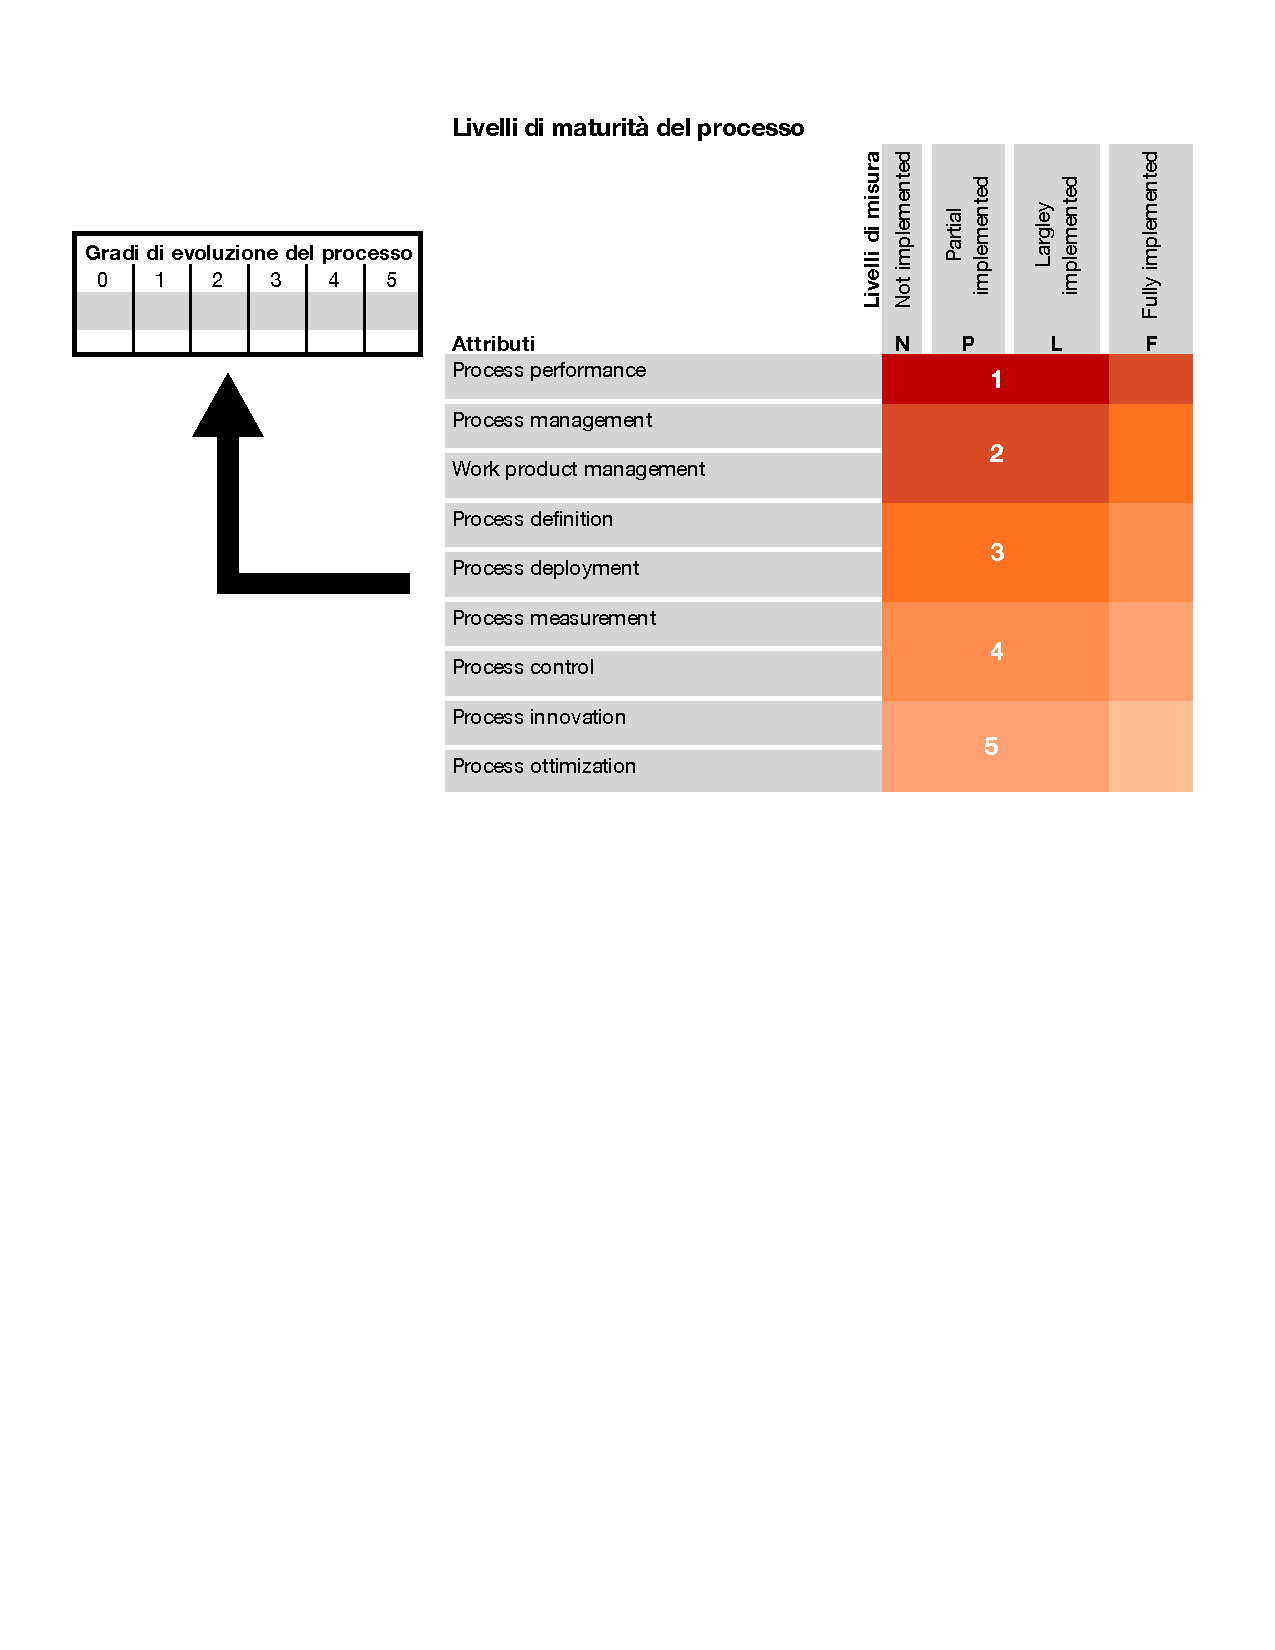
\includegraphics[scale=0.7]{images/ISOIEC15504.pdf}
	\caption{Riepilogo modello ISO/IEC 15504}
\end{figure}
\newpage

\subsection{Ciclo di Deming}
Il ciclo di Deming, noto anche come PDCA (dall'inglese \textbf{P}lan-\textbf{D}o-\textbf{C}heck-\textbf{A}ct), è un metodo di gestione iterativo suddiviso in quattro stadi ed utilizzato per il controllo del miglioramento continuo dei processi e dei prodotti. Esso permette, nello specifico, di migliorare gradualmente la qualità dei processi in termini di efficienza ed efficacia, ottimizzando l'uso delle risorse e misurando la loro conformità rispetto le aspettative. \\
La seguente immagine riporta le attività previste a tale scopo e ne segue una breve descrizione. 
\begin{figure}[htbp]
	\centering
	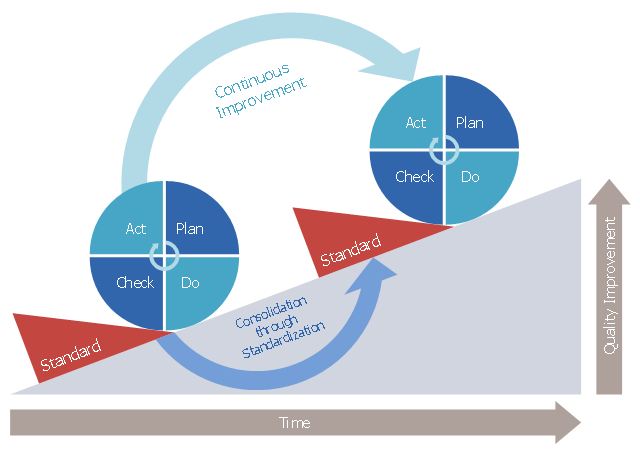
\includegraphics[scale=0.5]{images/pdca.png}
	\caption{Principio del miglioramento continuo secondo PDCA}
	
\end{figure}

\begin{itemize}
	\item \textbf{Plan}: prevede la definizione delle attività, scadenze, responsabilità e risorse atti a raggiungere e soddisfare degli obiettivi di miglioramento;
	\item \textbf{Do}: prevede l'esecuzione delle attività pianificate durante il periodo di pianificazione;
	\item \textbf{Check}: prevede la verifica dell'esito del processo in seguito all'attuazione delle strategie di miglioramento ed il confronto tra i risultati raccolti durante la fase Do e quelli attesi (specificati nella fase Plan) per stimare l'impatto effettivo del o dei miglioramenti apportati;
	\item \textbf{Act}: prevede l'attuazione delle strategie che hanno portato a dei miglioramenti. Nel caso i risultati attuali si distacchino da quelli previsti, si possono compiere delle azioni di correzione in seguito ad un'approfondita analisi delle cause di tale errore. 
\end{itemize}

\newpage
\section{ISO/IEC 9126}
Lo standard ISO/IEC 9126 definisce un modello dei requisiti qualitativi del Prodotto.
Il modello descritto si concentra in primo luogo sui tre punti di vista della qualità che esistono sul prodotto:
\begin{itemize}
	\item \textbf{Qualità esterna:} esprime il comportamento dinamico del software, in un determinato ambiente d'uso. In sostanza consiste nelle prestazioni e nelle funzionalità che il prodotto offre quando è in esecuzione;
	\item \textbf{Qualità interna:} esprime le proprietà statiche, cioè
	indipendenti dal contesto di esecuzione e uso. Sono direttamente misurabili ad esempio sul
	codice sorgente, pertanto senza la necessità di eseguire il software;
	\item \textbf{Qualità in uso:} esprime il livello con cui il prodotto si dimostra utile all'utente nel suo contesto d'uso. In altre parole rappresenta la capacità del prodotto di dare efficacia ed efficienza al lavoro dell'utente, a fronte di una sicurezza di utilizzo e di una soddisfazione nel far uso del prodotto.
\end{itemize}
\subsection{Modello per la qualità esterna ed interna}
Per la qualità esterna ed interna è definito un modello gerarchico formato da 6 caratteristiche principali e numerose sottocaratteristiche, tutte misurabili direttamente o indirettamente grazie all'utilizzo di metriche.
Le sei caratteristiche principali sono elencate di seguito:
\begin{itemize}
	\item \textbf{Funzionalità:} rappresenta la capacità del prodotto software di fornire funzioni che soddisfano le esigenze stabilite, sia esplicite che implicite, quando il software opera in un determinato contesto di utilizzo. Sottocaratteristiche notevoli sono l'interoperabilità e la Sicurezza, intesa come la capacità di proteggere le informazioni e i dati da accessi non autorizzati;
	\item \textbf{Affidabilità:} capacità di mantenere uno specificato livello di prestazione quando si opera in specificate condizioni. Sottocaratteristiche importanti sono la maturità e la tolleranza all'errore;
	\item \textbf{Efficienza:} capacità di fornire le funzioni richieste nel minor tempo possibile, sfruttando al meglio le risorse messe a disposizione;
	\item \textbf{Usabilità:} capacità del prodotto software di essere capito, appreso, usato e gradito all'utente, quando usato in contesti specificati. Una sottocaratteristica di rilievo è l'attrattiva;
	\item \textbf{Manutenibilità:} capacità del software di essere modificato e manutenuto. Per modifiche si intendono correzioni o adattamenti del software, negli ambienti, nei requisiti e nelle specifiche funzionali. Una sottocaratteristica importante è la testabilità, cioè la capacità di un software di consentire la verifica e di essere oggetto di test;
	\item \textbf{Portabilità:} capacità di poter essere trasferito da un ambiente di esecuzione all'altro.
\end{itemize}
\subsection{Modello per la qualità in uso}
Per la qualità in uso lo standard definisce una gerarchia separata, per enfatizzare il fatto che qui si considera non solo il prodotto software in sè, ma la relazione stretta tra esso e l'utente, nell'ambiente di utilizzo. Il modello è formato dalle seguenti quattro caratteristiche:
\begin{itemize}
	\item \textbf{Efficacia:} rappresenta la capacità di supportare un utente nel raggiungere i suoi obiettivi con accuratezza e completezza in un dato contesto;
	\item \textbf{Produttività:} la capacità di supportare un utente nello spendere l’appropriata quantità di risorse in relazione all’efficacia dei risultati da raggiungere; 
	\item \textbf{Soddisfazione:} la capacità di soddisfare un utente in un dato contesto d’uso;
	\item \textbf{Safety:} la capacità di raggiungere accettabili livelli di rischio di
	danni a persone, al software, ad apparecchiature, o all’ambiente operativo in un dato contesto d’uso.
\end{itemize}
\begin{figure}[htbp]
	\centering
	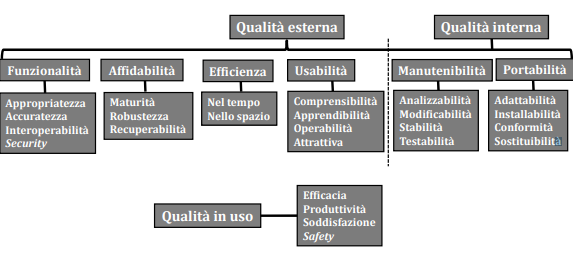
\includegraphics{images/gerarchiaQualitaProdotto.png}
	\caption{Riepilogo modello ISO 9126}
\end{figure}	
	
\end{document}
